\documentclass{grattan}
% add_to_dictionary: SRS SE.XPD.TOTL.GD.XS WDI SSNP NMS WPI DET SATs? ENG stds RCTs?

\newcommand*{\Vanish}[1]{}

\newcounter{superchapterfigure}
\newcounter{superchaptertable}
\newcounter{superchaptersection}

\newcommand{\addindentchap}[1]{%
	\setcounter{superchapterfigure}{\value{figure}}
	\setcounter{superchaptertable}{\value{table}}
	\setcounter{superchaptersection}{\value{section}}
	%\addtocontents{toc}{\protect\setcounter{temptocdepth}{\value{tocdepth}}}
	\addtocontents{toc}{\protect\setcounter{tocdepth}{1}}
	% So perhaps:
\addsec[#1]{\Large #1}  % [what appears in the toc]{what appears in the document}
	\setcounter{figure}{\value{superchapterfigure}}
	\setcounter{table}{\value{superchaptertable}}
	\setcounter{section}{\value{superchaptersection}}
	\addtocontents{toc}{\protect\setcounter{tocdepth}{0}}
}

\usepackage{multirow,bigdelim}

\newcommand\MyLBrace[2]{%
 \color{Orange}{ \left.\rule{0pt}{#1}\right]}\color{black}{\text{\hspace{1ex}#2}}}
 
 \newcommand{\tabitem}{\color{Orange}{~~\llap{\textbullet}~~}\color{black}}


\addbibresource{SchoolFunding.bib}
\GrattanReportNumber{2016-16}
\title{Circuit breaker: a new compact for school funding}
\author{Peter Goss and Julie Sonnemann}

\MONTH{November}  % compile time would be different
\YEAR{2016}

\hyphenation{NAPLAN}

\acknowledgements{%
This report was written by Peter Goss, Julie Sonnemann, and Kate Griffiths.
Carmela Chivers provided extensive research assistance and made substantial contributions to the report.

We would like to thank the members of Grattan Institute's School Education Program Reference Group for their helpful comments, as well as numerous government and industry participants and officials for their input.

The opinions in this report are those of the authors and do not necessarily represent the views of Grattan Institute's founding members, affiliates, individual board members reference group members or reviewers.
Any remaining errors or omissions are the responsibility of the authors.

Grattan Institute is an independent think-tank focused on Australian public policy.
Our work is independent, practical and rigorous.
We aim to improve policy outcomes by engaging with both decision-makers and the community.

For further information on the Institute's programs, or to join our mailing list, please go to: \textcolor{blue}{\url{http://www.grattan.edu.au/}}.

{\footnotesize
This report may be cited as:
Goss, P., Sonnemann, J., Griffiths, K., and Chivers, C. (2016). \emph{\mytitle}. Grattan Institute.

ISBN: 978-1-925015-96-6

All material published or otherwise created by Grattan Institute is licensed under a Creative Commons Attribution-NonCommercial-ShareAlike 3.0 Unported License\par
}
}
\begin{document}




\begin{overview}

A new approach can resolve Australia's fifty-year debate about how to fund our schools.
Commonwealth and state education ministers are meeting in two weeks' time to discuss a new funding model for 2018 and beyond.
They can agree to radical but achievable change.

This report proposes a compact for the needs-based funding system all main parties say they want.
It gives money to the schools that need it most.
And it kick-starts transformation of teaching and learning in all schools, investing in new roles for expert teachers to lift student performance. Critically, the compact does not require more Commonwealth funding, although some state governments may need to step up.

School funding needs a circuit breaker.
The needs-based model recommended by the 2011 Gonski Review was widely supported but not delivered in practice.
The trajectories in the 2013 Education Act are too slow: many under-funded schools will not be properly funded for decades, while other schools will still be over-funded at the \emph{end of the century}.

The legislated approach is also too costly.
It locks Australia into long-term funding growth rates that are too high given low wages growth.
In addition, Labor's promise that ``no school will lose a dollar'' entrenched decades of special deals done by both sides of politics.
To fund all schools according to need under this model, governments would have to spend around \$3.5~billion more every year.

The Coalition's 2016 Budget planned to cut the costs of the 2013 Act.
But the enacting the budget probably requires legislative change which have not been -- and may not be -- passed by Parliament.
The full details of the 2016 Budget plan are still unclear, but it appears
to create new problems.

The new compact shows how to deliver needs-based funding without the spending increases required by the 2013 Act.
With ongoing low inflation, school indexation rates are billions of dollars more generous than they need to be.
The compact seizes this historic opportunity.
It opens up large savings by reducing indexation rates to line up with wages growth.
It would then reallocate these funds to achieve needs-based funding by 2023.

Under the compact, very under-funded schools would be much better off compared to the 2013 model.
Chronically disadvantaged schools benefit the most.
Almost half of schools at or just below their targets would have slower funding growth, but they would maintain their purchasing power from today.
A small number of over-funded schools would lose money.
Compared to the 2016 Budget, most schools would be better off.
To avoid a similar mess in future we recommend greater transparency in funding.
These changes are vital to creating a school system that gives all children a fair chance in life.

Funding is not enough.
It must be accompanied by broader reforms to improve teaching and learning.
Investing in effective teaching does the most to lift student outcomes.
The compact redirects a big part of the savings relative to the 2013 Act to create two new teaching roles. \emph{Master Teachers} and \emph{Instructional Leaders} will work in and across schools to drive improvements in teaching effectiveness in their subject areas.

It is time to end the toxic funding debate so that we can focus on the debate that counts in this century: how do we equip our teachers to improve the learning of all students?
\end{overview}



\addchap{Recommendations}\label{chap:recommendations}
% This report outlines a new deal that aligns funding to need, and invests in teaching quality.
% It applies to both Commonwealth and state and territory governments.
% % The specific recommendations are:

\recommendation{Achieve needs-based funding by 2023}\label{rec:recommendation-1-achieve-needs-based-funding-by-2023}
Reduce indexation on school funding to be in line with education wages growth, and then re-allocate the savings to help every school reach at least 95~per cent of its Schooling Resource Standard (SRS) target by 2023.

\begin{itemize}
  \raggedright
    \item Index the SRS target in line with education wages growth, currently 2.5~per cent.
    \item Index annual funding at different rates so that all schools are brought into line with their SRS target more quickly.
    \begin{itemize}
        \item Index funding for under-funded schools at 3.6~per cent to help them catch up to their SRS target.
        \item Index funding for moderately over-funded schools at zero per cent so that over time their funding falls to their SRS target.
        \item Once schools are at or near their SRS target, indexation matches education wages growth, currently 2.5 per cent, to maintain purchasing power.
    \end{itemize}
    \item Provide top-up funds for schools very far below their targets -- because it will take too long to catch up via higher indexation rates alone.
    \item Decrease nominal funding year-on-year to a few highly over-funded schools.
    \item Apply these indexation rates to both Commonwealth and state government funding.
\end{itemize}

\oneraggedpage \pagebreak
\recommendation{Strengthen governance of school funding}\label{rec:recommendation-2-strengthen-governance-of-school-funding}

\begin{itemize}
    \item Establish an independent body to oversee school funding, including advising on the SRS formula and loadings, regularly reviewing indexation rates, and publicly reporting on funding outcomes.
    \item Through this independent body, review and improve the calculation of the SRS base rate, formula and loadings within the next 12 months and incorporate the findings into the new compact.
    \item Make the distribution of school funds more transparent by requiring all school systems to report publicly on the basis on which they allocate funds to schools.
\end{itemize}

\recommendation{Redirect the savings to invest in highly skilled teachers}\label{rec:recommendation-3-re-direct-the-savings-to-invest-in-highly-skilled-teachers-to-lift-the-effectiveness-of-the-workforce}
\begin{itemize}
    \item Establish new Master Teacher and Instructional Leader roles, with responsibility for driving improvement in teaching and learning.
\end{itemize}



\contentspage
\listoffigures

\chapter{The time is right for a new approach }\label{chap:the-time-is-right-for-a-new-approach}

\section{The political environment}\label{sec:the-political-environment}
School funding for 2018 and beyond is up for grabs.
The Commonwealth is negotiating with every state and territory government to agree on future resource allocations.
A new model must be determined by early~2017.

Whatever is decided is likely to require federal legislative change.
Parliamentarians will be forced to consider how much every school should receive, and why.

The Commonwealth Government has signalled that tough funding decisions may be on the table.
Commonwealth and state education ministers framed their September 2016 Education Reform Council meeting around funding and the need for trade-offs.

In a tight fiscal environment, prudent spending decisions are vital.
Yet budget pressures can actually create an opportunity for better policy.
Scarce resources can force governments to set priorities and focus on what matters most.

\begin{addsmallbox}[p]{How to read this report}{null}

This chapter gives a short overview on why a new approach to school funding is essential.
\Chapsref{chap:needs-based-funding-is-still-a-mess} to \topref{chap:indexation-on-school-funding-is-too-high} outline two big challenges: the mess of needs-based funding, and excessively high school indexation rates.

\Chapref{chap:the-new-compact-enables-two-big-reforms} answers these two challenges with a compact that strategically reallocates funds to have maximum impact.
The compact proposes reducing indexation to create big savings for two big reforms: needs-based funding by 2023 and a structural reform that better recognises highly skilled teachers as leaders of the profession.

\Chapref{chap:costing-the-compact} compares the costs of the various proposals.

A separate Technical Supplement details Grattan's financial model.
The financial model itself is available on the Grattan website.
\end{addsmallbox}

\section{School education outcomes}\label{sec:school-education-outcomes}
Australia's education outcomes, measured in international tests, have gone backwards since 2000.
Inequities between schools have grown.
Gaps in achievement are especially large for disadvantaged students. The principle that education can and must give every child a chance at a better life is far from being realised in practice.

Students from low socio-economic backgrounds make less progress than students from high socio-economic backgrounds. This is the pattern even for students with the same level of ability who achieve similar results early in their schooling life.\footcite{Goss2016Wideninggapswhat}

Grattan analysis published in 2016 showed how big the gaps are.
We used data from NAPLAN, Australia's first national standardised test and tracked the progress of the same students over six years.%
\footnote{NAPLAN is the National Assessment Program -- Literacy and Numeracy.
It is an annual test for Year~3, 5, 7 and 9 students.
Testing covers four domains: Reading, Writing, Language Conventions (spelling, grammar and punctuation) and Numeracy.}
We compared the progress of students in low, medium and high advantage schools.
Even when students have similar scores in Year~3, students in disadvantaged schools made \emph{one to two years less progress} than students in high advantage schools, as seen in \Vref{fig:widening-gaps}.
Bright students in disadvantaged schools lose the most.
They make two-and-a-half years less progress than their more advantaged peers.

These gaps hurt students' opportunities in life as well as Australia's future productivity and economic growth.

\begin{figure}
\captionsetup{oneside, margin={0pt,-1em}} % test
\caption{From the same Year~3 score, students in disadvantaged schools make much less progress to Year~9}\label{fig:widening-gaps}

\units{Equivalent year level, students with same Year~3 score (low, medium, high), school advantage, numeracy, Victoria, 2009--15}

\includegraphics[page=21]{atlas/Charts.pdf}

\source{Grattan analysis, \textcite[][Figure 14, p. 30]{Goss2016Wideninggapswhat}}
\end{figure}


This report seeks to provide a sensible proposal that can deliver funding where it can make the most difference.

\section{Why focus on school funding?}\label{sec:why-focus-on-school-funding}

Some question the value of increasing education funding further. Over the last 15~years Australia's school results got worse when funding increased.
Although Australian school funding is not particularly high by developed country standards, people are right to be concerned.
Some additional funding in Australia has been spent where it wasn't likely to do much for outcomes.

But poorly used funds in the past should not end the debate.
Freezing or indiscriminately cutting funding is not the answer.
Money spent well does matter.
Emerging evidence internationally shows that well targeted school funding can make a big difference.
And in Australia, recent investments in needs-based funding are working.

\subsection{Changes in spending over the last decade }\label{subsec:changes-in-spending-over-the-last-decade}
Australian spending on school education increased over the last decade, but student outcomes did not improve.
Whatever we did, it didn't work. And doing the same again is likely to have the same outcome.

Unfortunately, much of the extra funding went to areas that were unlikely to drive improvements in student learning. Between 2004-05 and 2013-14, government funding increased by \$10 billion in real terms.%
\footcite{Commission2016NationalEducationEvidence} Our analysis shows that about \$8 billion of this increase went to a mix of everyday items: rising student numbers, wage increases, and the ongoing costs of increased investments in government school buildings.%
\footnote{For further discussion, see \textcite{Goss2016SchoolFundingRose}.}
These investments might help to maintain the status quo but are unlikely to drive improvements in the classroom.
So it is not surprising that big funding increases did not lift outcomes.

\subsection{Ignore the hype: Australia is not a big spender in education }\label{subsec:ignore-the-hype-australia-is-not-a-big-spender-in-education}
\begin{figure}
\caption{Australian education spend is middle of the pack in comparison to GDP\label{fig:Aust-edu-spend-is-middle-of-pack}}
\units{School education spend as a per cent of GDP, 2013}

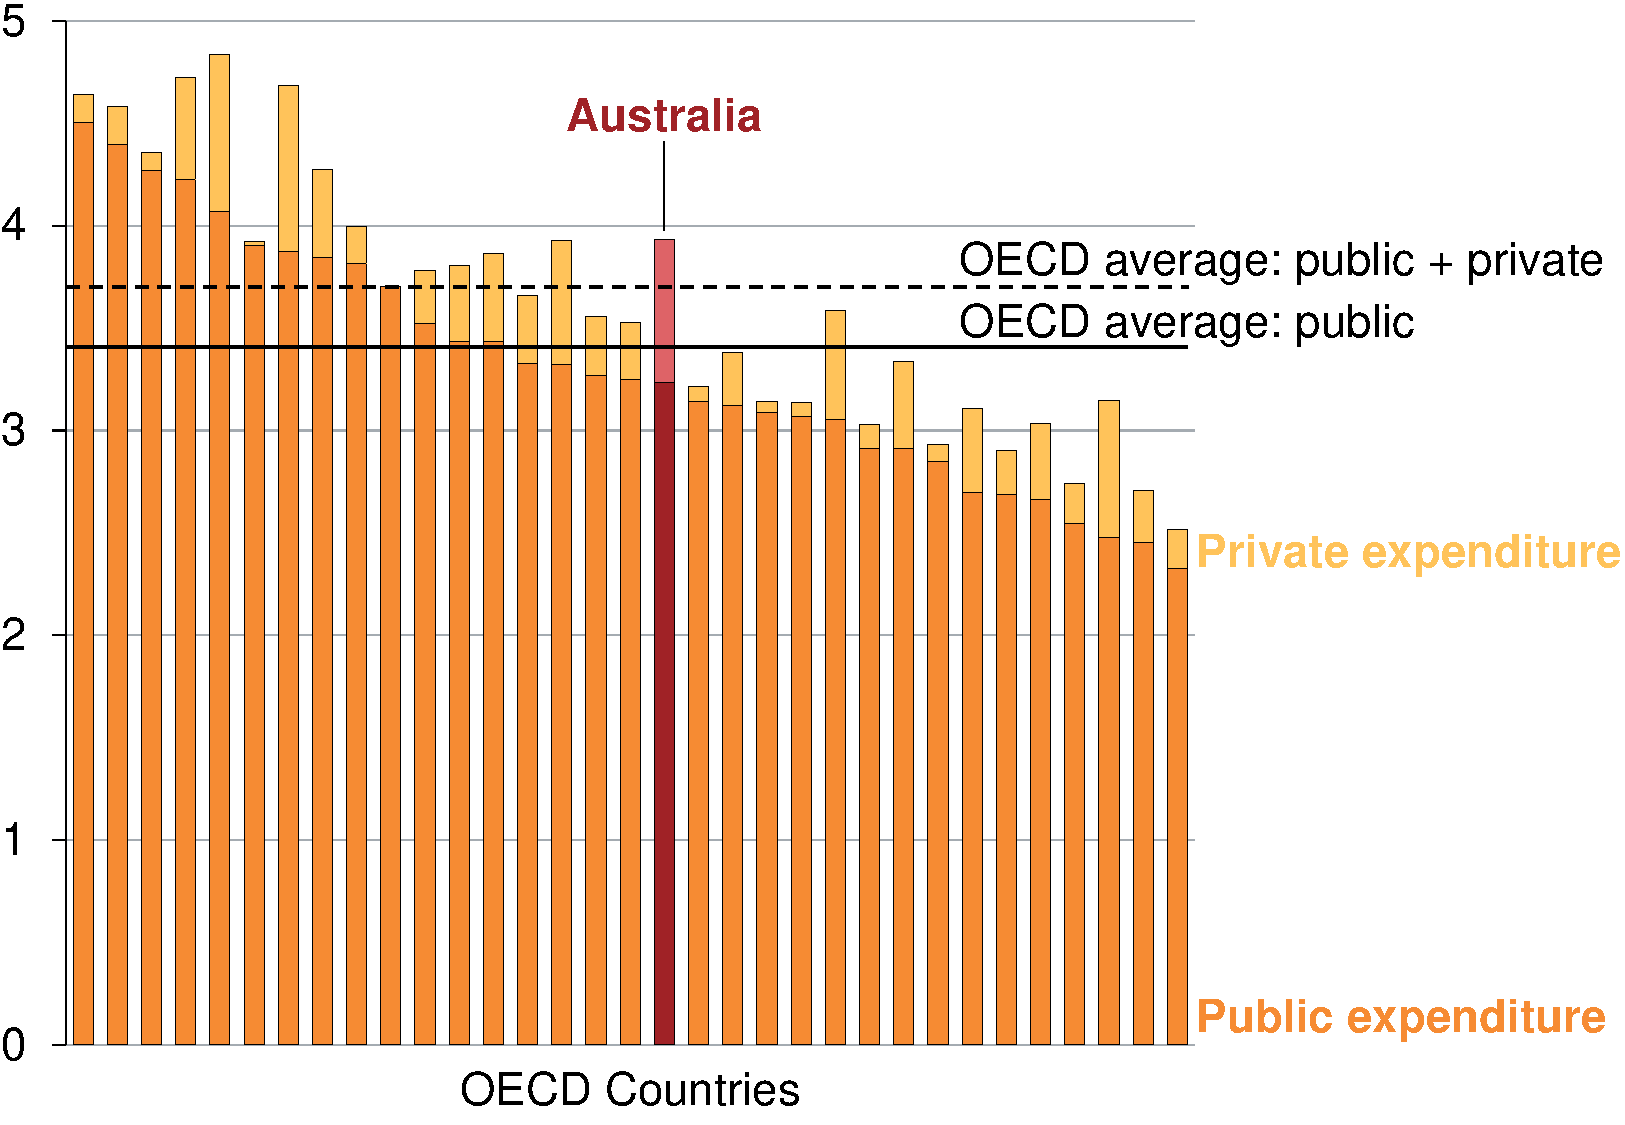
\includegraphics[page=1]{atlas/Charts.pdf}

\noteswithsource{OECD countries are ranked by public spend on education in 2013.}%
{Grattan analysis of \textcite[][207]{OECD2016EducationGlance2016}}
\end{figure}

On the other hand, Australia is not a particularly big spender on school education.
The claim that Australia is ``amongst the top of the pack'' in education spending is misleading.%
\footnote{Education Minister quoted from \textcite{Conifer2016GlobalEducationReport}.}
Relative to GDP, Australia's total spending on schools is only a little above the average of advanced economies (\Vref{fig:Aust-edu-spend-is-middle-of-pack}).
Government spending is a little less than the OECD average, while private spending is materially higher.

Until 2000, Australian governments consistently devoted a larger proportion of GDP to schools than other high income countries.
Since~2000, Australian governments have spent up to half a percentage point of GDP less than their peers.%
\footnote{\textcite{WorldBank2016WordDevelopmentIndicators}, WDI series SE.XPD.TOTL.GD.XS.}

\subsection{Emerging evidence shows investments in education can improve outcomes -- when spent well}\label{subsec:emerging-evidence-shows-investments-in-education-can-improve-outcomes}

Educational researchers have long contested how school funding affects student achievement, and this literature is reviewed in \Chapref{chap:appendix-2-do-extra-funds-improve-student-results}.

Simple statistical techniques that look at overall education funding levels and outcomes often find little relationship -- a conclusion that is then echoed in our political debates over school funding.

But using simple statistical techniques to assess the impact of funding fails to disentangle the influence of other factors.
Using stronger statistical tools, later researchers have re-analysed available data to show that ``money does matter after all'', as long as it is spent well.%
\footnote{\textcite[][13]{Hedges1994ExchangePartI} see also: \textcites{Greenwald1996EffectSchoolResources}{Krueger2003EconomicConsiderationsClass}.}

More rigorous research (mostly from the US and UK) on the impact of school funding takes advantage of natural experiments and randomised controlled trials in order to create a richer picture that separates the influence of funding, family background, and other factors on student outcomes.

One such natural experiment emerged out of the dramatic changes to education spending in the US that followed court-ordered school funding reforms from the 1970s.
It showed that students who received 10~per cent more funding across all schooling years as a result of these reforms stayed longer in school, were more likely to graduate, and earnt higher wages.%
\footcite{Jackson2016EffectsSchoolSpending}
In addition, the gap in test score outcomes between advantaged and disadvantaged students narrowed as a result of these reforms.\footnote{\textcite[][80]{Card2002Schoolfinancereform}: ten years after a reform, students in low-income districts had improved their test results by one-fifth of the original gap between low-income and high income districts, see: \textcite{Lafortune2016SchoolFinanceReform}.}

The effect on long-term outcomes was even stronger for students from low socio-economic backgrounds. \footcites{Card2002Schoolfinancereform}{Jackson2016EffectsSchoolSpending}{Lafortune2016SchoolFinanceReform}

Clearly, the distribution of spending can have a significant impact on whether we are getting the most from every dollar.
The fact that students from low socio-economic backgrounds tend to respond particularly strongly to funding increases suggests that targeting funding to the most educationally disadvantaged is a good starting point to ensure that money is well spent.

The idea makes sense. The cost of educating disadvantaged students tends to be higher given the additional barriers they face.%
\footcite{OECD2012EquityQualityEducation}
Socio-economic background has a large influence on student achievement.\footnote{\textcite{Hattie2008visiblelearningsynthesis}.}

\subsection{Schools must spend money wisely, and the policy settings must be right}\label{subsec:Schools-and-governments must spend money wisely}

More money alone will not guarantee better student outcomes.
It is not enough to target money to the most disadvantaged schools; each school must then use that money wisely.

School leaders need to be able to manage resources well -- no easy task.
Not only should funding go toward the right level of support from appropriately qualified personal such as counsellors, speech therapists, interpreters and community liaison officers -- but funding must also go to teaching practices that are demonstrably effective.

When this happens, the results can be remarkable.
Effective teaching is known to have the largest impact on student outcomes outside the home,%
\footcite{Hattie2008visiblelearningsynthesis}
and has been the subject of many previous Grattan Institute reports.%
\footnote{See previous reports at \textcolor{blue}{\url{https://grattan.edu.au/home/school-education/}}.}
Investments need to be made to help teachers make better use of evidence-based teaching practices.
In particular, the use of data, evidence, and feedback to adapt and improve teaching is has very large effects.%
\footnote{See \textcite{Goss2015TargetedTeachingHow}.}
Teachers also improve when they receive meaningful appraisal and feedback, with opportunities to observe others and share practices and ideas.%
\footnote{\textcite[][7]{Jensen2011BetterTeacherAppraisal}.
For a more specific discussion of the initiatives that work best for disadvantaged students and schools, see \textcite{OECD2012EquityQualityEducation}.}

For changes to school funding to be effective, however, governments must have the right policy settings in place too.
The level of system support, autonomy, incentives, career structures and other mechanisms all affect school leaders and teachers in their work with students. Targeted support programs can provide access to expertise, professional development, specialist staff, resources and more (for recent evaluations of Australian targeted programs, see \Vref{box:recent-programs-targeting-student-disadvantage-in-Australia-show-promising-results}). Getting these policy settings right is vital in order to improve teaching at scale.


To achieve improvement, the right amount of money is necessary but not sufficient.
This report therefore examines both how to improve the distribution of school funding, and how to enable it to be spent better in future.

\begin{smallbox}{Recent programs targeting student disadvantage in Australia show promising results}{box:recent-programs-targeting-student-disadvantage-in-Australia-show-promising-results}

There are few rigorous evaluations of programs targeting disadvantaged students and schools in Australia.%
\footcite{Commission2012SchoolWorkforce} However, some positive results are seen from the multi-billion dollar Australian Smarter Schools National Partnerships (SSNP) program since 2009, showing that targeted system support to schools can have positive effects.

The SSNP was a major initiative to improve the outcomes of low socio-economic students, with a range of different support programs in all states and territories.
For example, some programs invested in extra resources to attract the best leaders and teachers, others invested in teacher and school leader professional development.
Since the program ended, four statistical evaluations found positive effects on student achievement, especially in programs in Victoria and NSW.%
\footnote{More evaluations may have been undertaken but are not readily accessible.
Of the four evaluations cited, final evaluations are still to come given the impact of programs can take many years.}
%Carmela to check

In addition, a recent evaluation of a large NSW program \emph{(Early Action for Success)} for very disadvantaged schools found that investing in teacher capacity lifted student outcomes in the first three years of schooling.%
\footnote{\emph{Early Action for Success} is the NSW Department of Education strategy for improving literacy and numeracy in the first three years of primary school.
It is focused on the most disadvantaged government primary schools in NSW.}

A detailed summary of the program evaluations are included in \Chapref{chap:appendix-2-do-extra-funds-improve-student-results}.
\end{smallbox}

\chapter{Needs-based funding is still a mess}\label{chap:needs-based-funding-is-still-a-mess}

Australia is a long way from aligning school funding to student need.
Both main federal parties claim to support needs-based funding, but it is hard to see how either will achieve it.

This chapter gives an overview of current school funding arrangements, the needs-based funding principles that should be adopted, and how long it will take to align actual funding to target levels under current approaches. It also notes the need for new governance arrangements.

\section{The principles of needs-based funding}\label{sec:the-principles-of-needs based-funding}

The underlying aspiration of needs-based funding is that ``all students [should] have access to a high standard of education regardless of their background or circumstances''.\footcite[][xxxi]{Gonski2011ReviewFundingSchooling}
Consistent with this aspiration, each school should be funded at a level sufficient to provide a good education for their particular student mix.%
\footcite[][xxi]{Gonski2011ReviewFundingSchooling}
Since disadvantage, disability, language difficulties and other factors make it more challenging and expensive to educate some students, certain schools require additional resources and support to deliver them a quality education.
\footcite[][xxi]{Gonski2011ReviewFundingSchooling}

Any needs-based funding standard has two key components. First it sets a base rate of funding for students across the board.  Second, it calculates "loadings" for various forms of disadvantage. By combining these it sets a target level of funding for each school that takes into account the needs of its students.

But Australia has never had a coherent and nationally consistent approach for distributing funds across schools, sectors and states.
Historical levels of funding, rather than need, have influenced the funding that each school and sector actually receives. Decisions have typically been made through negotiations between governments, sectors and stakeholders, leading to inconsistent funding outcomes.

Moving from historically-driven funding to a needs-based funding standard involves two steps.
First, it reduces variance between schools, by increasing the funding of schools that are below their target, and reducing the funding of schools that are above.
Second, it moves the average level of funding for all schools to whatever has been set as the general level of funding for students.

\section{The recent history of needs-based funding}\label{sec:politics-has-got-in-the-way-of-good-policy}

School funding in Australia has grown up through a series of historical, often ad hoc, decisions. Special deals and promises that `no school will lose', made by both sides of politics, have compromised funding models.%
\footnote{Labor promised no school would lose a dollar in the introduction of the SRS model in 2013.
The Coalition made a similar commitment when it introduced its SES funding model in 2001.}
Once made, special deals are hard to wind back.
They tend to lock in an expensive and ineffective funding regime.

\subsection{The Gonski review proposed a new model}\label{subsec:the-gonski-principles-should-be-the-goal}

The 2011 Review of Funding for Schooling -- ubiquitously known as the Gonski review -- highlighted how the distribution of funding to Australia's schools over the past 40 years has tightened the link between aggregated social disadvantage and poor educational outcomes.\footnote{See \textcite{Boston2016WhatGonskiReally} for a recent summary of the review's findings and later developments.}
The report articulated the principles of a needs-based funding system.
It recommended a nationally consistent funding model for all schools, based on educational need and circumstance.%
\footcite[][xxi]{Gonski2011ReviewFundingSchooling}

The Review estimated a base rate of funding for all students that it argued was needed to deliver a good education.
It proposed loadings for disadvantaged students.
And it outlined a transition path to move towards the new levels of target funding.

\subsection{The Schooling Resource Standard was a step forward but implementation has been a challenge}\label{subsec:the-schooling-resource-standard-was-a-stepforward-but-needs-review}

The Labor Government of the day adopted several significant Gonski recommendations.
The \emph{Australian Education Act 2013} (Commonwealth) (`2013 Education Act') legislated that every school -- government or private -- would have a target rate of funding called its Schooling Resource Standard (SRS) amount.%
\footcite{2013AustralianEducationAct}
The SRS is a target level of government funding calculated to be sufficient for the school to achieve high quality outcomes (see \Vref{box:how-does-the-schooling-resource-std-work}).

\begin{smallbox}{How does the Schooling Resource Standard work?}{box:how-does-the-schooling-resource-std-work}

The SRS establishes a base rate of funding per student, then additional loadings for students and schools that need extra support to reach a basic academic standard.
Loadings are provided for low socio-economic status, disability, indigeneity, low English proficiency and rural and small schools.%
\footnote{For an overview of how the SRS model works see \textcite{Independent2014SRSFundingModel}.}

Government schools receive the full resource standard per student plus any additional loadings.
Non-government schools have their base funding adjusted to account for an estimate of parental capacity to contribute.%
\footnote{The parents of non-government schools are deemed to be able to contribute between 20 and 80 per cent of the SRS funding amount, depending on socio-economic status. \textcite{ABS2016SchoolsAustralia}.}

To account for increasing costs, the SRS base funding and loadings increase by 3.6~per cent a year.
The 2013 Education Act specifies this indexation rate at a fixed nominal amount, rather than linking it to an external benchmark.

The national SRS model calculates target funding for each school, and combines this to determine overall funding for school systems.
Participating states and Catholic systems have some flexibility to re-distribute funds to the schools within their system based on their own needs-based funding formulas. In practice this means there are still many different needs-based funding formulas in place.
\end{smallbox}

The SRS was not the first attempt to target resources according to need.
In the past, various Commonwealth programs provided additional funds to disadvantaged schools (outside of the school funding formula).
Some state and territory governments also had needs-based models in place, but these were not universal and they worked differently in different states.

The SRS was a significant step forward because it sought to establish one consistent formula based on need that could apply across all jurisdictions and sectors (with some appropriate flexibility).

But in practice, the SRS fails to do so. There are problems in how the SRS is calculated (see \Cref{subsec:Selecting-an-appropriate-funding-base-rate}).
And subsequent policy decisions were not consistent with the principles of needs-based funding.

The Labor Government's policies were often described as the `Gonski reforms', but they did not fully reflect the principles of the Gonski review. Prime Minister Julia Gillard committed that no school would lose a dollar under any changes.%
\footcite[][xxi]{Gonski2011ReviewFundingSchooling}
Consequently, new arrangements embedded a number of special deals and historical funding quirks. As a result, schools with comparable student needs can receive different funding, for no policy reason other than history.%
\footcite{Gallash2013SecretGonskiDeals}

\subsection{Transitional arrangements to the SRS have stalled }\label{subsec:transitional-arrangements-to-the-srs-have-stalled}

Since 2013 the federal and state governments have agreed to transitional arrangements designed to enable schools to reach 95~per cent of their SRS target by 2019.%
\footnote{For Victoria it is 2021.} %
There have been two major stumbling blocks.

First, most of the Commonwealth funding to lift funding from current levels to 95~per cent of their SRS target was to be provided in 2018 and 2019, the final two years of the agreement struck in 2013.
This funding never eventuated.%
\footnote{The Labor government commitment to funding for 2018 and 2019 was outside the Budget forward estimates at the time.
Following the 2013 election, the Coalition Government committed to only the first four years (2014 to 2017).}

Second, the picture is complicated by the special deals done with different sectors and states.

Despite these set-backs in the national approach, some states and sectors have continued to advance more targeted needs-based funding through their own local models, but this not a long-term answer.%
\footnote{Cooperation between Commonwealth and state governments is essential to achieve a sustainable, sector-blind model because the Commonwealth government contributes most of the funding to non-government schools, while state and territory governments contribute most of the funding to government schools.}
Needs-based funding remains a mess.

\section{Funding is still not directed to where it can have the greatest impact}\label{sec:current-situation-funding-is-still-not-directed-to-where-it-can-have-the-greatest-impact}

Despite recent efforts, funding is still not allocated according to educational need and is unlikely to be so for a long time.
Most school systems get less funds than their target calculated to be sufficient for the aggregate needs of their students. This section outlines how far schools are from their target.

Given data limitations, it is not possible to analyse individual schools in the Government and catholic sectors in any detail. However school level data is available for independent schools and authorities, and contrary to popular belief, we show that many independent schools are underfunded relative to their target funding levels.


\begin{figure}[!p]
\caption{Funding levels differ by state and sector but most systems are funded less than their targets}\label{fig:funding-levels-differ-by-state-and-sector}
\units{Combined government funding as a per cent of SRS, by state, 2016}

\includegraphics[page=2]{atlas/Charts.pdf}

\noteswithsource{* ACT Independent schools receive combined government funding at over 150~per cent of SRS}%
{Grattan school funding model, based on analysis of data published by the Commonwealth Department of Education and Training.}
\end{figure}

\subsection{Most school systems are underfunded relative to their targets}\label{subsec:most-school-systems-are-under-funded}

As \Vref{fig:funding-levels-differ-by-state-and-sector} shows, most school systems are on average funded below even 95~per cent of their SRS targets.

\begin{figure}
\caption{It would cost governments \$3.5 billion more in 2016 to fund all schools to at least 95 per cent of SRS}\label{fig:cost-of-funding-all-schools-to-95-per-cent}

\units{Estimated gap to 95 per cent of SRS, by sector by state, 2016 (\$ billions)}
\includegraphics[page=4]{atlas/Charts.pdf}
\noteswithsource{Full details of how we estimated the needs-based funding gap are provided in the Technical Supplement.}%
{Grattan school funding model based on analysis of data published by the Commonwealth Department of Education and Training.}
\end{figure}
%\addtolength{\textfloatsep}{-0.6\baselineskip}


Funding all school systems at 95 per cent of SRS would require an additional \$3.5 billion a year, if nothing else changed.
Most of the additional funds would go to government schools in NSW, Victoria and Queensland, as shown in \Vref{fig:cost-of-funding-all-schools-to-95-per-cent}.
\cleardoublepage


\subsection{Many individual schools are under-funded }\label{subsec:most-schools-are-under-funded}

Many individual schools are funded much less than their targets.

Most individual government and Catholic schools appear to be underfunded relative to even 95~per cent of their SRS targets (this can be inferred given that these systems in most States are underfunded in aggregate). But detailed data on individual schools in these systems is difficult to obtain, so in this section we rely on the best available public information which is on individual independent schools (only).

Our analysis shows many independent schools are under-funded relative to their SRS target. Some individual independent schools are only funded at 40 to 60~per cent of their targets (see \Vref{fig:some-independent-schools-well-below-SRS-target}).
Collectively, independent schools in 2014 were under-funded by about \$400~million.
The amount of under-funding for most independent schools is larger than the amount of over-funding of a few independent schools.

The under-funding of many independent schools is at odds with many public perceptions. But much of the growth in independent schools over the last two decades served families from low-income backgrounds.\footcites{KingndTheStructureandFunding}{Buckingham2016OneSchoolDoes}

\begin{figure}
\caption{Some independent schools receive far too little funding, some receive far too much\label{fig:some-independent-schools-well-below-SRS-target}}

\units{Number of independent school approved authorities, by level combined government funding as a per cent of SRS, 2014}

\includegraphics[page=3]{atlas/Charts.pdf}

\source{Grattan analysis of Questions on Notice from \textcite{SenateSQ15000888}, SQ15-000888}
\end{figure}




%\afterpage{\addtolength{\textfloatsep}{0.6\baselineskip}}
%\cleardoublepage

\subsection{Some schools are extremely over-funded}\label{subsec:some-schools-are-extremely-over-funded}

Only a small number of schools are over-funded, but many millions of dollars of excess funding flows to them.

To estimate over-funding for individual schools we again rely on the detailed data that is (only) available for the independent sector. We estimate that a small number (representing less than one per cent of all schools) and 30 per cent of independent school students) received \$215 million more than their SRS target in 2014.\footnote{Just 142 out of 831 approved authorities for independent schools receive combined government funding above SRS\@.}

Over time, the over-funding is substantial -- about \$2~billion over the next 10 years.
This is wasteful and inefficient.

Even within the group of over-funded independent schools, just 28~schools receive more than half the over-funding, seen in \Vref{fig:more-than-half-the-overfunding-goes-to-28-schools-above-150pc-of-SRS}. At the very top end, some independent schools receive nearly three times their per student SRS target -- and still get automatic annual increases in per student funding (see \Vref{box:one-stark-example-of-overfunding} for an example).

\begin{figure}
\caption{A tiny number of schools receive nearly than half of the over-funding dollars\label{fig:more-than-half-the-overfunding-goes-to-28-schools-above-150pc-of-SRS}}
\units{Distribution of over-funding in 2014 (\$ millions), by level of combined government funding as a per cent of SRS, independent schools}

\includegraphics[page=7]{atlas/Charts.pdf}
\source{Grattan analysis of data reported in \textcite{Knott2016Morethan150} and Questions on Notice from \textcite{SenateSQ15000888}, SQ15-000888}
\end{figure}
\begin{smallbox}[H]{One stark example of over-funding}{box:one-stark-example-of-overfunding}
One independent school in Sydney received nearly \$8,000 per student in combined government funding in 2014 compared to a target funding level of under \$3,000.

It is hard to see why: 97~per cent of its students are from the top half of the socio-economic distribution, and in 2016 its fees ranged from \$12,000 to \$18,000.
The school does not appear to enrol an unusually high number of students with disability, or from a non-English speaking background.
And yet under the current model, each year this school would get 3~per cent more Commonwealth funding, or \$160 extra per student.

Every government dollar this school receives above its funding target is not being spent on a school that needs it more.
\end{smallbox}

\phantom{.}

\phantom{.}

\pagebreak[4]

Some individual schools in the government and Catholic sectors are probably also over-funded, but individual school data is not publicly available to estimate this.

The only government or Catholic \emph{system} (as opposed to individual schools) that appears to be funded above its SRS target is the ACT public school system.
In 2017 it is projected to receive combined government funds of 112~per cent of its target.%
\footnote{\textcite{SenateSQ15000244}.
This high level of funding is driven by generous funding from the ACT Government, rather than from the Commonwealth.}

\begin{pagesmallbox}{How we use the SRS target in this report}{box:use-of-SRS-target-in-this-report}
Despite problems, the SRS targets are still a step in the right direction. For this report we use the current SRS targets as the best available estimate of schools' needs-based funding requirements. Until they are improved, they should remain the point towards which all schools should move.
Under the compact, we make a conservative assumption that governments should aim to get under-funded schools to 95~per cent of current SRS targets.
\end{pagesmallbox}

\section{The current targets are a large unfunded liability}\label{sec:needs-based-funding-is-now-a-large-unfunded-liability}

On any view, many systems and schools are funded much less than what is needed according to current definitions.

But a large part of the cost of needs-based funding depends on the definition of the base rate of funding for students.
More work is needed to determine an appropriate base rate of funding.
For now, there would be few regrets from moving to 95~per cent of the SRS as currently defined.

\subsection{Commitments to needs-based funding}\label{subsec:commitments-to-needs-based-funding}

Both major parties have signed up to the principles of a national needs-based funding model.%
\footnote{The SRS formula was enshrined in 2013 legislation passed by Labor, and the principle of needs-based funding was reiterated in the Coalition's 2016 Budget, which stated that ``additional funding will be based on the principles of being needs based, stable, simple, fair, transparent'' {\textcite[][No.~2, p.~80]{Treasury2016BudgetPapers2016}}.}
Needs-based funding is currently defined by the SRS targets. But current funding arrangements fall well short of delivering even 95~per cent of these targets. We estimate that to lift all schools to 95~per cent of SRS, around \$3.5~billion of extra funding would be needed each year.%
\footnote{There have been many different estimates of the size of the needs-based funding gap. For example, the Parliamentary Budget Office estimated for the Labor party that funding the final two years of Gonski would cost \$4.5~billion.
This estimate maintains that no school will lose a dollar. See:
\textcite{PBO2016PostElectionReport}.}
The gap between needs-based funding as currently defined, and actual funding, has become an unfunded liability for the taxpayer.

\subsection{The size of the gap between actual funding and the current definition of needs-based funding }\label{subsec:siz-of-the-gap-between-actual-funding-and-the-current-definition}

The size of that liability depends on how much schools vary from the SRS target, and the base rate of funding under the SRS

Using the (only) available data on independent schools, most of the cost of moving to a needs-based funding model results from providing additional resources to schools that are substantially under-funded according to any plausible base rate of funding.

\Vref{fig:getting-to-95pc-cheaper-more-targeted-than-100pc} shows that lifting the funding to students at very under-funded schools to 95~per cent of the SRS standard will cost \$400~million.
By comparison, it would cost another \$200~million to lift those students -- and others in schools already at 95~per cent -- to 100~per cent of the SRS standard.

Data is not publicly available to determine how much of the cost of shifting to a needs-based funding model for government and Catholic schools is a consequence of providing funds to severely underfunded schools as opposed to incrementally increasing funding for many more schools already close to the target.

\begin{figure}[p]
\caption{Getting to 95~per cent of SRS is cheaper and much more targeted than getting to 100~per cent\label{fig:getting-to-95pc-cheaper-more-targeted-than-100pc}}
\units{Combined government funding as a per cent of SRS, by cumulative number of students, independent schools only, 2014}

\includegraphics[page=5]{atlas/Charts.pdf}

\source{Grattan analysis of \textcite{SenateED0572} Question No. ED0572\_15}
\end{figure}




\subsection{Selecting an appropriate funding base rate} \label{subsec:Selecting-an-appropriate-funding-base-rate}

Going the last mile to move all students up from 95 to 100~per cent is very expensive and less targeted.
The value of doing so is questionable.
A small funding increase for most schools across the board will probably deliver less return than targeting funding to those materially below their SRS target.
Emerging evidence shows that funding tends to have a greater impact when it is targeted to educational need, as discussed in \Vref{subsec:emerging-evidence-shows-investments-in-education-can-improve-outcomes}.

The base SRS amount represents the resources required to support a student with minimal student disadvantage. There are real problems in how it has been calculated.


The Gonski panel attempted to define the base SRS by reference to the funding of a group of high-performing schools in which at least 80~per cent of students were above the national minimum standard (NMS) in NAPLAN.%
\footnote{\textcite{Justman2013WhatsWrongGonski}, cited in \textcite{SenBackn.d.GovernmentSenatorsDissenting}.}
There are a number of problems with this approach:

\begin{itemize}[itemsep=1.2ex]
\item The benchmark is based on student achievement levels, when it is far more meaningful to measure how students are progressing (improving) over time.%
\footnote{For further discussion of student progress, see \textcites{Goss2016Wideninggapswhat}{Jensen2010MeasuringWhatMatters}.}
\item The benchmark drew on a very limited number of high achieving schools (that were most likely also high socio-economic schools) which may not accurately represent the amount of funding required for a good education.
\item The benchmark is based on Australia's national minimum standards of student achievement, which are far too low.\footnote{See \textcite{Goss2016Wideninggapswhat} \citetitle{Goss2016Wideninggapswhat} recommending these national minimum standards be raised or scrapped.}
\item The 80~per cent threshold is itself arbitrary -- why not, say, 75~per cent or 85~per cent?
\end{itemize}

In any case, the Gonski panel was unable to calculate this standard accurately. It only obtained limited data on the costs of the nominated high-performing schools, and was unable to produce a detailed analysis of their costs.%
\footnote{\textcite{NCA2014TowardsResponsibleGovernment}.}

As the Government moved to implement the Gonski recommendations in 2013, it did not set up an independent panel to revise the SRS standard as the Gonski Review had recommended. It is unclear if further work was done to improve the rigour of the SRS base rate. It is clear that the government revised the preliminary loadings developed by the Gonski panel. But it did so through consultations with stakeholders, rather than the deep, robust data analysis that was recommended. The consultation process has been criticised by many.%
\footnote{The \textcite{NCA2014TowardsResponsibleGovernment} highlights criticisms of the quality of data underlying the disadvantage loadings, with large amounts of data missing, inconsistent or inaccurate. Final loadings were seen as diluting the principles of the Gonski review (\textcite[][42]{Connors2015ImperativesSchoolsFunding}).
The disability loading in particular requires more work, given definitional differences across the states.}

The overall outcomes of the SRS model -- which implies that nearly every school system in the country is underfunded -- should be revisited, given the limited data analysis that appears to have been undertaken.

And given that it projected an additional \$3.5~billion was needed to reach just 95~per cent of target funding levels (see \Vref{fig:cost-of-funding-all-schools-to-95-per-cent}), it is not surprising that governments have aimed for 95~per cent of the target rather than 100~per cent of the calculated SRS\@. This report follows that lead.

Lifting the funding of significantly under-funded schools as a first priority will cause few regrets.
Even if loadings are calculated differently, or a lower base rate was used, these schools will still be allocated substantially more money under a needs-based system.

\pagebreak[3]
\section{Transitioning to target levels of funding}\label{sec:The-current-transition-arrangements-will-take-a-long-time}

The current transition arrangements will take a long time to align schools to their SRS target.

Under the provisions of the 2013 Education Act, schools that are below their SRS target are supposed to catch up to their target through higher indexation rates (see \Vref{box:higher-indexation-rates-help-some-schools-catchup-faster}).

\begin{smallbox}{Higher indexation rates help some schools catch up faster under legislation}{box:higher-indexation-rates-help-some-schools-catchup-faster}

The 2013 Education Act sets the rate of indexation for all SRS \emph{targets} at 3.6~per cent.
The Act also defines three rates of indexation for annual Commonwealth funding%
\footcite{2013AustralianEducationAct} which differ depending on a school's current funding relative to its SRS target:\footnote{In practice, funding for most schools is allocated to their Approved Authority (\eg~the state government or Catholic schools authority) in an aggregated way.
Funding allocations for schools below SRS are netted off against the funding for schools above SRS within an Approved Authority.}

\begin{itemize}[leftmargin=1.0em]
\item Schools below their SRS target  receive annual funding indexation of 4.7~per cent per student.
This is higher than the indexation rate for SRS targets, helping them to catch up to target;
\item Schools at their SRS target  receive annual funding indexation of 3.6~per cent per student, keeping them on target in terms of Commonwealth funding.
\item Schools above their SRS target  receive annual funding indexation of 3~per cent per student.
This is lower than the indexation rate for SRS targets, bringing them back to target slowly;

\end{itemize}

Each state and territory also determines its own approach to funding and indexation, creating a complex arrangement of separate bilateral agreements with the Commonwealth.%
\footnote{As one example, the agreement between the Commonwealth and NSW specifies that NSW contributes 3~per cent indexation plus 35~per cent of needs-based top-up payments for schools below SRS (with the Commonwealth contributing the remaining 65~per cent of top up payments).}

Indexation rates are discussed further in \Chapref{chap:indexation-on-school-funding-is-too-high}.
\end{smallbox}

Yet even with the higher indexation rate, some schools below SRS will take a very long time to catch up to their targets (see \Vref{fig:some-underfunded-schools-still-below-target-even-in-a-decade}).

\begin{figure}
\caption{Under the 2013 Education Act, the most under-funded schools will still be funded well below their SRS target even in a decade}\label{fig:some-underfunded-schools-still-below-target-even-in-a-decade}

\units{Combined government funding as a per cent of SRS, by sector and year}
\includegraphics[page=6]{atlas/Charts.pdf}

\noteswithsource{The most under-funded government school system is in Victoria, and the most under-funded Catholic system is in the Northern Territory.
The sample for independent schools was taken from the 100 most under-funded schools in Australia in 2017.}
{Grattan school funding model, based on analysis of data published by the Commonwealth Department of Education and Training.}
\end{figure}

It will also take too long to align over-funded schools with the SRS target.
The 2013 Education Act determined that for schools above their SRS targets, annual funding would grow at a slower rate than the average SRS target for all schools (see \Vref{box:higher-indexation-rates-help-some-schools-catchup-faster}).
This rate was designed to narrow the gap between actual and target funding over time.

But for these schools, even with a slower growth rate, we estimate that it will take more than a hundred years for actual funding to align with target funding, as shown in \Vref{fig:overfunding-will-persist-until-end-of-century}.

\begin{figure}
\caption{Under the 2013 Education Act, over-funding will persist until the end of the century\label{fig:overfunding-will-persist-until-end-of-century}}

\units{Value of combined government funding above SRS by calendar year, independent schools (2016 dollars, \$ millions)}
\includegraphics[page=8]{atlas/Charts.pdf}

\noteswithsource{It is likely that some individual government and Catholic schools are also over-funded relative to SRS, but school-level data about funding in relation to SRS is only publicly available for independent schools.}%
{Grattan analysis of Questions on Notice from \textcite{SenateSQ15000888}, SQ15-000888}
\end{figure}
\afterpage{\cleardoublepage}
%\afterpage{\cleardoublepage}
\oneraggedpage\pagebreak[4]
\section{The Commonwealth's proposal to equalise funding across states could create perverse outcomes}\label{sec:equalise-funding-across-states}
Recently the Commonwealth Education Minister Simon Birmingham indicated he wants to remove any disparities in Commonwealth funding among states.%
\footcite{Balogh2016WildInequalityGonski}
If this happens in isolation from other changes, it could have perversely benefit some well-funded students and reduce funding to those who need it most.

\begin{figure}
\caption{Commonwealth funding for government schools varies greatly by state}\label{fig:funding-is-highly-variable-by-sector-and-state}

\units{Commonwealth funding as a per cent of SRS, projected for 2018 under 2013 Education Act, government schools only}

\includegraphics[page=12]{atlas/Charts.pdf}
\noteswithsource{Line indicates Commonwealth funding of 16.8\% of SRS for government schools which would be the new funding level for all states from 2018 under the Commonwealth Government's proposed equalisation approach}{Grattan school funding model, based on analysis of data published by the Commonwealth Department of Education and Training; and Question on Notice from Senate Committee: Education and Employment  (2015--2016), SQ15-000703.}
\end{figure}

As \Vref{fig:funding-is-highly-variable-by-sector-and-state} shows, Commonwealth contributions to government schools vary substantially by state. It is unclear what the \mbox{Government's} proposed equalisation approach would do, but under one scenario the Commonwealth would fund all states at 16.8~per cent of SRS from~2018.%
\footnote{The 2015-16 Budget figures include an assumption that government school systems will each receive 16.8 per cent of the Schooling Resource Standard from the Commonwealth in 2018, \textcite{SenateSQ15000703}, Question No. SQ15-000703.}

In the absence of other changes, this would lead to inappropriate outcomes for some students.

For example, Western Australian government schools currently receive the least from the Commonwealth, at 13.0~per cent of SRS\@. If equalised up to 16.8~per cent, they would receive more Commonwealth funding. But in aggregate the students are already funded at 100~per cent of SRS (see \Vref{fig:funding-levels-differ-by-state-and-sector}). Additional Commonwealth funding would be more than is needed to provide a quality education.

By contrast, Northern Territory government schools are currently under-funded relative to SRS, despite generous Commonwealth funding above 23~per cent of SRS\@. This is because funding from the Territory government has historically been low. But, if equalised down to 16.8~percent, NT would lose nearly a quarter of its Commonwealth funding.
NT students would be even more underfunded relative to SRS\@.

Under equalisation, the three biggest states Queensland, NSW and Victoria would also receive less than specified in the 2013 Education Act.
Reducing Commonwealth funding to currently under-funded school systems is likely to be resisted fiercely, especially when government schools in these three states are funded less than Catholic and independent sectors.

\section{Better governance is required}\label{sec:the-srs-formula-must-be-reviewed-and-governance-arrangements-strengthened}

% \afterpage{
% \begin{minipage}[0.99\textheight]{\linewidth}
% \phantom{.}
% \vspace{036pt}
% \setlength{\parskip}{0.6\baselineskip}
% \begin{verysmallbox}[H]{How we use the SRS target in this report}{box:use-of-SRS-target-in-this-report}
% For this report we use the current SRS targets as the best available estimate of schools' needs-based funding requirements.
% Despite problems, the SRS targets are still a step in the right direction.
% Until they are improved, they should remain the point towards which all schools should move.
% Under the compact, we make a conservative assumption that governments should aim to get under-funded schools to 95~per cent of current SRS targets.
% \end{verysmallbox}
% \vspace{0.5\textheight}\phantom{.}
% \end{minipage}
% }

As the previous sections show, needs-based funding is a mess.
Cleaning it up must begin with better governance.
We propose three key steps that must go alongside any attempt to move schools toward needs-based funding targets.

\begin{enumerate}[leftmargin=1.5em]

\item Establish an independent body, as suggested in the Gonski review, to calculate funding targets, recommend funding arrangements, and report publicly on funding. An independent body is needed to take the politics out of school funding decisions, to make them transparent, and to facilitate consistent evaluation of the impact of new funds.

\item Ensure that the SRS formula is the right one. There are methodological issues with both the needs-based loadings (the extra amounts that schools receive for higher levels of student need) as well as the base SRS amount (which represents the basic resources required to support a student with minimal student disadvantage), as discussed above in
\Vref{subsec:Selecting-an-appropriate-funding-base-rate}.

\item Strengthen requirements for public reporting of system decisions on school funding. The public have the right to know how significant amounts of taxpayer funds on schooling are being allocated. At present there are few requirements and little is known about how systems are re-distributing funds at a local level.
\end{enumerate}

\chapter{Indexation on school funding is too high}\label{chap:indexation-on-school-funding-is-too-high}

\Chapref{chap:needs-based-funding-is-still-a-mess} shows that Australia is still far from achieving needs-based funding.
This chapter explores a different problem that seems unrelated but is vital to the argument of this report. Given the low inflation environment, the Commonwealth's fixed rate of indexation of school funding is too high. Addressing these two problems together can solve both, as discussed in \Chapref{chap:the-new-compact-enables-two-big-reforms}.

\section{School funding should grow in line with wages growth}\label{sec:school-funding-should-grow-in-line-with-wages-growth}

School funding is indexed each year so that inflation does not erode its real value.
Because school budgets are so large, indexation rates matter to overall budget outcomes.

This report proposes that per student funding should broadly be indexed to wages growth in the education sector (more specifically to the Education Wage Price Index).%
\footnote{The Technical Supplement to this report includes a more detailed discussion of alternative options. It explains it is more appropriate to index to wage growth rather than CPI or Education CPI\@.
It also explains that it is more appropriate to index to the Education and Training (Public and Private) WPI rather than general WPI\@.
Although the two are very similar, the Education WPI is more closely related to the wage costs that schools are likely to face.}
Wages comprise about 80~per cent of government school operating costs.\footnote{Grattan analysis based on \textcite{Commission2016ReportGovernmentServices}.
There is no precise breakdown of the remaining 20~per cent of expenditure, but it includes purchased services which are largely wages, as well as supplies which are likely to track overall inflation.
See Technical Supplement for further discussion.}

\begin{figure}
\caption{Education wages growth has slowed in line with other prices}\label{fig:edu-wages-have-slowed-over-past-few-years-as-inflation-has-come-down}
\units{Per cent change from previous calendar year as at financial year end}
\includegraphics[page=10]{atlas/Charts.pdf}
\noteswithsource{Wage price indices for Australian education and training, public and private, total hourly rates of pay excluding bonuses; consumer price index is for all groups.}
{\textcites{ABS2016ConsumerPriceIndex}{ABS2016WagePriceIndex}}%, 6401.0, CPI Series A2325847F; \textcite{ABS2016WagePriceIndex}, 6345.0 WPI Series A2603451V.}
\end{figure}

\section{Legislated Commonwealth indexation rates are too high }\label{sec:legislated-commonwealth-indexation-rates-are-too-high}

Unusually, the Gillard Government's 2013 Education Act set fixed indexation rates of 3.6~per cent for school funding, rather than pegging them to the Education Wage Price Index or another index linked to actual economic conditions.

Since these rates were set in 2013, the economy has slowed, and inflation and wage growth have slowed along with it, as \Vref{fig:edu-wages-have-slowed-over-past-few-years-as-inflation-has-come-down} shows.

At present, annual growth in the Education Wage Price Index is at 2.5~per cent.
There are good reasons to believe that education wages growth will remain this low for many years.
Inflation looks likely to remain low: markets are pricing the 10-year inflation rate at 1.6~per cent (as at September 2016).%
\footnote{\textcite{RBA2016G3InflationExpectations}.
See Technical Supplement for further discussion.} %
And Education WPI tends to track the Consumer Price Index (CPI) -- albeit 1~percentage point higher.%
\footnote{In the decade to 2014, Education WPI broadly tracked movements in general CPI, albeit 1.0~per cent higher and with roughly a six month lag. The current lower level of the Education WPI is consistent with lower CPI, which fell from its typical level of 2.5-3.0~per cent between 2004 and 2014 to its current rate of 1.0-1.5~per cent.}

Since education wages growth is now low (at around 2.5 per cent), the Commonwealth's fixed indexation rates of 3 to 4.7~per cent are too high (see \Vref{fig:legis-locks-in-indexation-rates-too-high}).

The problem is even more pressing because low wages growth will reduce bracket creep and future income tax revenues, putting even more pressure on the Commonwealth budget.%
\footnote{\textcite{Daley2015FiscalChallengesAustralia} \citetitle{Daley2015FiscalChallengesAustralia}.}

\begin{figure}
\caption{Small changes to indexation rates add up over time}\label{fig:legis-locks-in-indexation-rates-too-high}

\units{Funding per student, for a hypothetical school that receives government funding equal to 100 per cent of SRS in 2016 (nominal, \$ thousands)}
\includegraphics[page=9]{atlas/Charts.pdf}

\noteswithsource{For the sake of illustration, annual funding per student for this hypothetical school is set at \$10,000 in 2016. (1) Under the 2013 Education Act, Commonwealth funding for a school at SRS is indexed at 3.6\%. For the sake of illustration, this figure assumes that state funding would also be indexed at 3.6\%. (2) Projected Education Wage Price Index of 2.5\% is a Grattan assumption based on current Education WPI and 10 year inflation forecasts, see Technical Supplement for more detail.}
{Grattan analysis.}
\end{figure}

\section{The 2016 Budget set new indexation rates that create new problems}\label{sec:the-2016-budget-set-new-indexation-rates-that-create-new-problems}

The 2016 Commonwealth Budget proposed a new school funding indexation rate of 3.56~per cent for three years from 2018 to 2020.
There is no official commitment to apply different rates to different schools, but this appears likely.%
\footnote{The sentiment in the Budget Papers appears to indicate that different rates may apply given that additional funding will be distributed based on need, according to \textcite[][No.~2, p.~80]{Treasury2016BudgetPapers2016}: ``\emph{Total school funding will be indexed by an education sector specific index of 3.56~per cent, with an allowance for changes in enrolments.
The additional funding will be based on the principles of being needs based, stable, simple, fair, transparent\dots}''.}
But it is unclear how individual schools will be affected, or whether the previous structure of differentiated indexation will apply.

The 2016 Budget did not commit to indexation rates beyond 2020, and it remains unclear what will happen from 2021 onwards.
One scenario is that indexation will revert back to the 2014 Budget proposal to index funding in line with CPI, and therefore more slowly than wages growth.

The 2016 Budget proposal has three major problems:

First, indexation rates of 3.56~per cent are higher than is needed for the next 4 years for schools or systems that are at their SRS target.
If CPI continues to be around 1.5~per cent, then Education WPI growth is likely to be closer to 2.5~per cent through to 2020.

Second, if indexation then reverts to CPI from 2021, it will be too low.
Because wages typically grow faster than CPI, effective school resourcing would fall.%
\footnote{Indeed, if education funding had grown at CPI for the decade to 2013, Australia's education funding would have been in the bottom quarter of OECD countries as a function of GDP, rather than in the middle (see \Vref{fig:Aust-edu-spend-is-middle-of-pack}).}

\begin{figure}[p]
\caption{The Commonwealth is either on a problematic funding pathway (2016 Budget) or an expensive one (2013 Education Act)}\label{fig:neither-indexation-pathway-is-desirable}

\units{Projected Commonwealth school funding (nominal, \$ billions)}

\includegraphics[page=11]{atlas/Charts.pdf}
\source{Grattan school funding model, based on analysis of data published by the Commonwealth Department of Education and Training.}
\end{figure}

Third, it is unclear to which schools the 3.56~per cent indexation rate will apply. Schools and systems need to know exactly what differential rates might apply, if any, to understand how they will be affected.

The 2016 Budget provides a further \$1.2~billion over four years relative to the 2014 Budget,\footnote{The 2014 Budget proposed that Commonwealth school funding would grow at CPI plus enrolments from 2018 onwards.} but does not explain how the funds would be distributed.
It proposes no credible path for closing the needs-based funding gap.

\section{Neither the 2013 nor the 2016 path works, and political problems loom}\label{sec:neither-the-2013-nor-the-2016-path-works-and-political-problems-loom}

Neither the 2013 Education Act nor the 2016 Budget offers a sensible pathway for Commonwealth school funding.
The legislation sets indexation rates that are now too high.
The 2016 Budget saves money but creates new problems.
It appears not to close the gap towards needs-based funding targets and may well make matters worse (\Vref{fig:neither-indexation-pathway-is-desirable}).

The 2016 Budget promised school education savings to Treasury of about \$1.7~billion in 2018-21 relative to the 2013 Education Act.
But it is doubtful whether these will be delivered given the political realities.

Legislation is probably required to amend some of the funding guaranteed by the 2013 Education Act.
The 2013 Act defines Commonwealth indexation rates for most schools.\footnote{The indexation rates in the legislation apply specifically to `participating schools', which includes all non-government schools as well as government schools in the three participating jurisdictions of NSW, SA and ACT.}
On some legal interpretation, the Act entitles these schools to funding as indexed.
Whatever the strict legal entitlement, the 2013 funding allocations are likely to be provided, despite the intent of the 2016 Budget, unless the Senate passes amendments to the Act.

Given that Labor and the Greens went to the 2016 election promising more money for schools, the Senate is unlikely to agree to  legislative change to reduce funding and move away from needs-based funding.

Furthermore, the 2016 Budget proposals will be difficult to sell to the states because lower indexation rates would disproportionately affect schools -- mostly government schools -- that are currently below their SRS target.

A political impasse looms.
The Commonwealth needs a solution that all stakeholders will accept.
The next chapter outlines a way forward.

\chapter{The new compact enables two big reforms}\label{chap:the-new-compact-enables-two-big-reforms}

Overly high indexation of school funding creates a big opportunity for reform.
Lowering the rates would free up significant savings to finally deliver on  needs-based funding (see \Vref{fig:compact-is-only-approach-that-gets-schools-to-geq-95pc-of-target}).

This chapter proposes a new compact that redistributes funds from low priorities to high priorities.
Both Commonwealth and state governments must contribute for it to work.
It will redistribute savings, primarily from reduced indexation, to achieve two big reforms.

\begin{figure}
\caption{The new compact is the only approach that gets schools to at least 95~per cent of their SRS target target}\label{fig:compact-is-only-approach-that-gets-schools-to-geq-95pc-of-target}

\units{Aggregate government funding to schools as a per cent of SRS target}

\includegraphics[page=14]{atlas/Charts.pdf}

\noteswithsource{(1) Includes needs-based funding top-up payments but not investment in workforce reform. (2) Assumes that indexation reverts to CPI after 2021, although this is not clear in the 2016 Budget papers.
\\ Note that the SRS targets are lower under the new compact because they are indexed at a lower rate than in other scenarios. Funding above 100\% is excluded as it does not contribute to closing the needs-based funding gap. Under the new compact all schools reach at least 95\% of SRS -- schools that are already funded between 95\% and 100\% of SRS will retain their current funding levels in real terms.}%
{Grattan school funding model, based on data published by the Commonwealth Department of Education and Training.}
\end{figure}

\begin{itemize}
\item
  \textbf{Part~A: Deliver needs-based funding} by 2023; and
\item
  \textbf{Part~B: Invest in highly skilled teachers} to drive improvements in all schools.
\end{itemize}

These two reforms are circuit breakers, at a time when there is a high risk that governments will slide back into an unhelpful blame game over funding.

Part~A and Part~B complement and reinforce one another.
Realigning school funding to need (Part~A) is long overdue.
But funding is not enough.
Reforms to school funding must be accompanied by broader reforms to improve teaching and learning (Part~B).

It is widely recognised that teachers make the biggest difference to student learning.
Yet current workforce structures neither encourage nor enable our most talented teachers to develop others around them.
Our initiative in Part~B introduces two new roles to enable highly skilled teachers to help spread evidence-based practices across schools.
The new initiative will not solve everything.
But it can spark real change in how we value teaching and help create a far more professional sector.

The teaching reform is \emph{in addition} to needs-based funding. All schools can opt-in to benefit from new expert teacher roles, but still have discretion over any extra needs-based funding.

The compact we propose is based on the principles outlined in \Vref{box:Six-principles-behind-the-new-compact}, which should be widely supported.

\begin{verysmallbox}{Six principles behind the new compact:}{box:Six-principles-behind-the-new-compact}
\begin{enumerate}[leftmargin=1.7em]
\item \textbf{Alignment to need:}
Funding should be better targeted according to student need, given the costs of educating some students is higher than others.

\item \textbf{Maintenance of schools' purchasing power:}
The compact maintains the real value of funding for schools over time.

\item \textbf{Fiscal responsibility:} Target funding to where it can make the most difference, and minimise the overall cost to government budgets.

\item \textbf{Transparency:}
All stakeholders must know that funding is going to where it is needed.

\item \textbf{Effectiveness:}
What matters is what happens in the classroom. New workforce structures help spread effective teaching.

\item \textbf{Cooperation:} Both Commonwealth and state governments must work together to help schools reach their SRS targets.
\end{enumerate}
\end{verysmallbox}

\section{Our approach to modelling school funding}\label{sec:how-does-report-model-school-funding}

Grattan Institute has built a model to estimate current and future funding.
Drawing on publicly available funding information from Senate Estimates Questions on Notice, we create a funding baseline for 2014 to 2017 by sector and by state, with more granular information for independent schools.
The model uses this baseline to project future funding changes under various policy settings.%
\footnote{We project funding on a year-by-year basis for each sector within each state, with Commonwealth and state funding estimated separately.
The year-on-year funding calculations combine projected enrolment changes with an appropriate per student funding indexation rate.
The applicable rate depends on whether the prior year's total government funding for each group of schools was at, above or below its SRS target.}

We make six key assumptions in modelling the new compact proposal:
\begin{enumerate}%[leftmargin=1.25em,itemsep=-0.4ex]
\raggedright
\item Index the SRS target in line with education wages growth, currently 2.5~per cent
\item Index annual funding at different rates so that all schools are brought into line with their SRS target more quickly
\item All states and the Commonwealth set the same indexation rates
\item Split the contributions to needs-based top-up funding (Part~A): Commonwealth 65~per cent, states 35~per cent
\item Split the contributions to teaching reform (Part~B): Commonwealth 35~per cent, states 65~per cent
\item Our modelling for the legislated pathway reflects the 2013 Education Act only.%
\footnote{It does not include the National Education Reform Agreement (2013).}
\end{enumerate}

A Technical Supplement provides further detail on the key assumptions and the structure of the model.%
\footnote{The Technical Supplement and the model itself are available on the Grattan Institute website at \textcolor{blue}{\url{http://grattan.edu.au/home/school-education/}}.}

\addindentchap{Part~A: Deliver needs-based funding}\label{chap:part-a-achieving-needs-based-funding}

\section{Overview of key concepts}\label{sec:overview-of-key-concepts}

Our proposal significantly reduces indexation to create big savings that can be redistributed to help all schools catch up to 95 per cent of their SRS funding targets.

The indexation rates the 2013 Education Act would be reduced for both target and actual per student funding.
Doing so generates significant savings for reallocation to under-funded schools.
This report calls these `top-up payments'.

The compact also winds back funding for highly over-funded schools, overturning the idea that no school will lose a dollar.
This change will only affect a small number of schools, but it is important symbolically and helps to remove a source of future arguments.

Combined, these changes enable all schools to reach between 95 and 100~per cent of their SRS target by 2023.
This is a huge step forward and helps to realise the Gonski aspiration of sector-blind, needs\nobreakdash-based funding.
It does so within the same funding envelope as the 2016 Budget, and at lower cost than the 2013 Education Act, as shown in \Vref{fig:most-savings-from-reducing-indexation}.%

\begin{figure}
\caption{The compact creates savings, primarily by reducing indexation, and reallocates them to two big reforms}\label{fig:most-savings-from-reducing-indexation}

\units{Projected Commonwealth savings compared to 2013 Education Act (nominal, \$~billions)}

\includegraphics[page=13]{atlas/Charts.pdf}

\source{Grattan school funding model, based on data published by the Commonwealth Department of Education and Training.}
\end{figure}


\section{The four steps to achieve needs-based funding}\label{sec:details-of-the-four-steps-to-achieve-needs-based-funding}

This section explains each of the changes required to enable needs-based funding:\footnote{All changes apply on a per student basis, so no school is penalised for higher or lower student enrolments in future.}

\begin{enumerate}
\item
  Reduce indexation of the SRS target;
\item
  Reduce indexation of annual school funding;
\item
  Reduce funding to highly over-funded schools; and
\item
  Provide top-up payments to highly under-funded schools.
\end{enumerate}

\subsection{Reduce the indexation rate of the SRS target}\label{subsec:i-reduce-the-indexation-rate-of-the-srs-target}

In a low inflation environment, school costs grow more slowly, so the funding target should grow more slowly as well.
The SRS target per student should grow in line with education wages growth, since this drives most of the annual increases in costs for schools.%
\footnote{We propose aligning SRS target indexation to wages growth from 2017 onwards since wages growth has already dropped.
All other changes proposed in the compact are from 2018 onwards when current funding arrangements expire.
See Technical Supplement for further information.}

Today, annual growth in the Education Wage Price Index is about 2.5~per cent and is expected to stay low for some time (\Vref{sec:school-funding-should-grow-in-line-with-wages-growth}).

It costs less to lift all schools to their target funding levels if the SRS target is lower.
As \Vref{fig:cost-funding-all-schools-to-target-SRS-reduced-under-compact} shows, the national SRS target in 2027 would be about 9~per cent lower under our compact than under legislation.
The change makes needs-based funding much cheaper to achieve.

\begin{figure}
\caption{The cost of funding all schools to their SRS target is much lower under the compact than under the 2013 Education Act}\label{fig:cost-funding-all-schools-to-target-SRS-reduced-under-compact}

\units{Estimated cost of funding all schools to their SRS target (nominal, \$billions)}

\includegraphics[page=15]{atlas/Charts.pdf}

\source{Grattan school funding model, based on data published by the Commonwealth Department of Education and Training.}
\end{figure}


\subsection{Reduce indexation rates on annual funding}\label{subsec:ii-reduce-indexation-rates-on-annual-funding}

The compact also reduces indexation of annual funding -- the increase in funding a school receives each year as it moves towards its SRS target.

The compact proposes different rates of indexation, depending on a school's current funding level compared to its SRS target.%
\footnote{The changes we propose to indexation of annual funding apply from 2018 when current funding arrangements expire.} Indexation remains high for under-funded schools to help them catch up. Funding is frozen for over-funded schools so that over time their resourcing falls to their SRS target. Schools at or near SRS are indexed at wages growth.

Applying these different indexation rates will move all schools closer to their targets over time, as shown in the chart on the right hand side of \Vref{fig:compact-realigns-all-schools-compared-to-budget-and-legislation}.

The use of different indexation rates is consistent with the approach in the 2013 Education Act. Indexation rates vary for the same reason: to gradually move all schools closer to their SRS target.

But the compact uses lower rates of indexation than in the 2013 Education Act because wages growth is now lower.
The difference generates most of the compact's savings -- about \$2~billion over four years for the Commonwealth -- 72 per cent of its total savings (\Vref{fig:most-savings-from-reducing-indexation}).

\begin{figure}
\caption{The compact applies different rates of indexation to different schools to help realign all schools to their target}\label{fig:compact-realigns-all-schools-compared-to-budget-and-legislation}
\units{Projected school funding versus 2015 SRS target}

\includegraphics[page=16]{atlas/Charts.pdf}

\noteswithsource{Illustrative examples of how school funding would grow under different scenarios for schools that in 2015 were funded at 60, 80, 100, 120 or 120 per cent of SRS, using a simplifying assumption that annual funding indexation rates is the same for states as for the Commonwealth.
\\ The 2013 Education Act scenario (LHS) includes annual indexation rates of 4.7\%, 3.6\% and 3.0\% for schools below, at or above SRS, respectively.
\\ The 2016 Budget scenario (middle) makes the simplifying assumption that all schools receive the same rates of annual indexation: 3.56 per cent for calendar years 2018 to 2020, then CPI from 2021 onwards.
\\ The new compact scenario (RHS) uses the indexation rules described in this chapter, and includes top-up funding and reductions for highly over-funded schools. It does not include workforce reform.}
{Grattan analysis; 2016 Budget; 2013 Education Act}
\end{figure}

\begin{table}
\caption{Indexation rates under the 2013 Education Act and the new compact}\label{tbl:compare-rates-of-indexation-under-Education-Act}

\begin{tabularx}{\linewidth}{p{0.25\linewidth}rR@{}lR@{}l@{ }}
%
\toprule
\phantom{.} & & \textbf{Education Act (2013)} & & \textbf{New compact} & \textsuperscript{\textdagger} \tabularnewline
\midrule
\multicolumn{2}{l}{\textbf{Target SRS indexation}}       & 3.6\%                 & & 2.5\%\tabularnewline
\null                                                    & \tabularnewline[-1ex]
\multicolumn{2}{l}{\textbf{Commonwealth annual funding}} &                       &  \tabularnewline
                                                         & Above SRS             &  3.0\%                        & & 0\%\tabularnewline
                                                         & 100\% SRS             &  3.6\%                        & & 2.5\%\tabularnewline
                                                         & 95-99\% SRS           &  4.7\%                        & & 2.5\%\tabularnewline
                                                         & \textless{}95\% SRS   &  4.7\%                        & & 3.6\%\tabularnewline
\null                                                    & \tabularnewline[-1ex]
\multicolumn{2}{l}{\textbf{States annual funding}}       &                       & \tabularnewline
                                                         & Above SRS             & 3.0\% &\textsuperscript{\(*\)} & 0\%\tabularnewline
                                                         & 100\% SRS             & 3.0\% &\textsuperscript{\(*\)} & 2.5\%\tabularnewline
                                                         & 95-99\% SRS           & 3.6\% &\textsuperscript{\(*\)} & 2.5\%\tabularnewline
                                                         & \textless{}95\% SRS   & 3.6\% &\textsuperscript{\(*\)} & 3.6\%\tabularnewline
\bottomrule
\end{tabularx}
{\footnotesize\itshape\begin{itemize}[itemsep=0ex,leftmargin=1em]
\item[\textdagger] In the new compact, SRS indexation reduces in 2017 and annual funding indexation from 2018.
\item[\(*\)] The 2013 Education Act specifies Commonwealth funding indexation, not state funding indexation.
We make a single set of assumptions about the indexation contributed by states, consistent with recent trends in DET data (see \Chapref{chap:appendix-3-contributions-of-commonwealth-and-state-governments}).
The compact proposes new indexation rates that are the same for all states and the Commonwealth from 2018.
\end{itemize}}
\source{2013 Education Act; Grattan school funding model, based on data published by the Commonwealth Department of Education and Training.}
\end{table}

\begin{smallbox}{How do individual schools fare under the compact compared to the 2013 Education Act and the 2016 Budget?}{box:how-do-individual-schools-fare-under-compact-compared-to-legis-2016-budget}

The impact of the compact relative to the 2013 Education Act and the 2016 Budget differs across schools.

\textbf{Seriously under-funded schools} (around 20~per cent of all schools) will be much better off.
This is a core objective of the compact: to target funding more intensively to the schools where it can make the biggest difference.

\textbf{Moderately under-funded schools} (about 30~per cent of all schools) will be slightly better off.

\textbf{Schools close to or at their targets} (45~per cent of all schools) will have slower funding growth.
Slower growth for these schools provides more funds for the most disadvantaged schools.
Schools close to their target maintain their purchasing power compared to today, and many will increase it.
By definition they already have enough resources to meet their students' needs

\textbf{Moderately over-funded schools} (about two per cent of all schools) will keep their nominal funding, but lose real resources over six years.

\textbf{Significantly over-funded schools} (around 100 schools, less than one per cent of all schools) will receive less funds per student year-on-year.
\end{smallbox}

In summary, the compact identifies three categories of school whose annual funding would be indexed at different rates:

\textbf{Schools at or just below their SRS} receive annual funding indexation of 2.5~per cent (in line with expected wages growth).
Under the 2013 Education Act, schools at their SRS get 3.6~per cent, and those just below get 4.7~per cent.%
\footnote{`Just below' SRS refers to schools between 95 and 100~per cent of SRS\@.
Adjusting their indexation to 2.5~per cent reflects our goal of getting all schools to 95~per cent of SRS, rather than 100~per cent.}

Because the indexation rate for funding (2.5~per cent) is the same as the indexation rate for the target SRS, once a school reaches its target, it stays at that level of funding.

\textbf{Schools well below their SRS} (below 95~per cent) receive a boosted indexation rate of 3.6~per cent -- which is above the 2.5~per cent rate that applies to all SRS targets.
This higher rate of indexation helps to move them closer to their target.%
\footnote{A higher rate of indexation for under-funded schools (relative to the indexation of SRS targets) is consistent with the current structure of legislated indexation (where schools below SRS get annual funding indexation of 4.7~per cent compared to 3.6~per cent indexation of the SRS target).}

\textbf{Schools above their SRS} receive no indexation of annual funding, in order to bring them back to their SRS target more quickly than under legislation.
When schools above SRS get back to their target, their funding is indexed at the same rate as other schools at SRS\@.
Freezing funding (with no nominal growth) reduces resourcing in real terms; but the impact is at least muted when inflation is low.

\Vref{tbl:compare-rates-of-indexation-under-Education-Act} summarises the changes to indexation rates for both Commonwealth and state and territory governments.

\subsection{Reduce funding to highly over-funded schools}\label{subsec:iii-reduce-funding-to-highly-over-funded-schools}

The compact would further reduce funding for schools that are well above their SRS, given that freezing funding will not return them to target funding levels by 2023.%
\footnote{Schools funded more than 116~per cent of SRS will not return to SRS by 2023 even if funding is frozen.}
Less than 100 schools are in this situation, less than one per cent of all schools, although they teach about five per cent of all students.

For these schools, we reduce funding year-on-year to return them to their SRS target by 2023.
They will lose money per student.
For most of these schools the funding decrease required is less than 5~per cent of their government funding each year for six years.%
\footnote{For 28 schools funded above 150\% of SRS funding would be reduced further, between 5-15~per cent per year. But this is a reduction in their \emph{government} funding not their \emph{total} funding. It does not apply to fees, which typically provide most of the budget for such schools.}

\subsubsection{Small but symbolically important savings }\label{subsubsec:small-but-symbolically-important-savings}

The savings from freezing indexation for all schools above SRS and reducing funding for highly over-funded schools together represent only 13~per cent of the total Commonwealth savings.
But these measures are important, helping to unwind some of the special deals of the past and align all schools to their target within a reasonable timeframe.%
\footnote{See, for example, the call by the Business Council of Australia to ``urgently phas[e] out all the side deals that were done to keep in place the promise that no school would be worse off.'' \textcite{Westacott2016FutureEducation}.}

\subsection{Provide top-up payments for very under-funded schools}\label{subsec:iv-provide-top-up-payments-for-highly-under-funded-schools}

Many schools are so under-funded that they will not reach their SRS target within any reasonable timeframe, even with a boosted annual indexation rate of 3.6~per cent.
They require top-up payments to reach their SRS target by 2023.

Needs-based top-up payments and workforce reform are the compact's two categories of new spending.

We calculate that all schools below about 90~per cent of their SRS target in 2016 will need this extra top-up funding to reach 95~per cent of their target by 2023.

We assume the Commonwealth will foot 65~per cent of the bill for needs-based top-up payments, while states pay the remaining 35~per cent.%
\footnote{For our costings of the compact, it was necessary to estimate the split in spending between Commonwealth and states.
We used this split because it was agreed by the Gillard Government as part of the National Education Reform Agreement negotiations, and also appeared in the 2013-14 Budget papers.}

We propose that needs-based top-up payments are phased in over six years, for two reasons.
First, if schools were to receive the entire amount bringing them up to their SRS target in one or two years then some would get a very large one-off boost in funding -- more than they could be expected to manage and spend well in a year.

Second, six years is the earliest that the spending can be afforded, given the aim of staying within the funding set out in the 2016 Commonwealth Budget.

\subsection{State contributions}\label{subsec:some-state-governments-will-need-to-step-up}

Under the compact, closing the national needs-based funding gap requires significant contributions from state governments as well as the Commonwealth.
The compact requires both levels of government to apply the same indexation rates set out in this report, as well as to contribute top up funding.

To meet these requirements, will each state government need to commit more funds than currently budgeted?
It is difficult to tell, given the opaqueness of state funding decisions.
Whether individual states need to contribute more will depend on what funding growth rate they are applying today and how far away their schools are from their SRS targets.
This is discussed further in \Chapref{chap:costing-the-compact} and in \Chapref{chap:appendix-3-contributions-of-commonwealth-and-state-governments}.

\section{Getting resourcing right is only the first step -- broader reforms are needed to teaching and learning}\label{sec:getting-resourcing-right-is-only-the-first-step-broader-reforms-are-needed-to-teaching-and-learning}

These changes to achieve needs-based funding are more than worthwhile on their own.
Yet many will rightly say that needs-based funding alone will not produce the improvements to teaching that our most disadvantaged students urgently require, or indeed that all Australian students deserve.

The next section -- the second part of the compact -- explains why another portion of the savings should be used to achieve a second (additional) reform: making the most of our highly skilled teachers.

With all schools being properly resourced under Part~A of the compact, Part~B applies to all schools.

\addindentchap{Part~B: Invest in highly skilled teachers}\label{chap:part-b-investing-more-in-highly-skilled-teachers}

To get the biggest impact from every dollar spent, we should invest in effective teaching. Evidence overwhelmingly shows that, outside the home, effective teaching has the most impact on student outcomes.%
\footcites{Hattie2008visiblelearningsynthesis}{McKenzie2005Teachersmatterattracting}{OECD2009CreatingEffectiveTeaching}

Yet we lack the right system structures and approaches to spread the use of evidence-based teaching practices in schools.
Our best teachers can lift the effectiveness of the whole workforce, but they often remain isolated with heavy teaching loads in their own classrooms.

The compact proposes a structural change to help address this issue by creating two expert teaching roles. These positions open up the skills of expert teachers, enabling them to coach and develop other teachers in their school and region. Every sector would be entitled to apply for these positions. It is only one of many reforms needed to lift teaching quality, but it is important.%
\footnote{For discussion of other reforms to improve teaching effectiveness see previous reports by the Grattan Institute at \textcolor{blue}{\url{http://grattan.edu.au/home/school-education/}}.}

The teaching initiative is \emph{in addition} to the needs-based funding reforms.
Schools can opt-in to benefit from expert teacher roles, on top of any extra needs-based funding they receive under the new model.%
\footnote{In our modelling we assume the Commonwealth will foot 35~per cent of the bill for this teaching initiative, while states pay the remaining 65~per cent. This is the reverse split of Part~A of the compact where we assume the Commonwealth pays 65~per cent and states pay 35~per cent.}

\section{The way teaching is organised needs to change}\label{sec:the-way-teaching-is-organised-needs-to-change}

It is widely known that teaching practice in Australia can and must improve.%
\footcites{Goss2015TargetedTeachingHow}{Jensen2010WhatTeachersWant}{Jensen2011BetterTeacherAppraisal}{Santiago2011OECDReviewsEvaluation}
A \citeyear{Commission2016NationalEducationEvidence} review by the Productivity Commission emphasised the lack of evidence-based teaching practice in our classrooms. \footcite{Commission2016NationalEducationEvidence} This long standing problem partly stems from the culture in schooling.
While every teacher is responsible in theory for using evidence to improve his or her teaching, it is no-one's day job to make sure it happens in practice.
The system historically allowed everyone to do their own thing behind closed doors.%
\footcite{Dinham2008TeachingTalentBest}
While this is changing, there is still a long way to go in many schools.%
\footnote{The introduction of the \emph{Australian Professional Standards for Teachers} has been an important step in making explicit the elements of effective teaching, including the need to work together to improve teaching in school settings.}

In Australia, the last day of a teaching career can look a lot like the first: with a regular teaching load and little professional collaboration with colleagues. The most talented teachers tend to have little chance to influence teaching beyond their classroom -- their capacity to help others is not utilised.

Change is needed. Teachers are known to teach more effectively when they work together, using observation and feedback to assess and critique each other's work.%
\footnote{See various studies by \textcites{Timperley2007TeacherProfessionalLearning}{Yoon2007ReviewingEvidenceTeacher}{Blank2009EffectsTeacherProfessional}{Desimone2009ImprovingImpactStudies}{Veen2012WhatMakesTeacher}, and previous Grattan reports on feedback: \textcites{Goss2015TargetedTeachingHow}{Jensen2011BetterTeacherAppraisal}.}
Teachers collective self-efficacy -- a group of teachers' shared belief in their ability to improve student learning -- substantially improves student outcomes.%
\footnote{\textcite{Hattie2009VisibleLearningArticle} John Hattie cites an effect size of 1.57 for teachers collective self-efficacy.}
In this light, the role of expert practitioners in guiding collaboration and team discussions is vital.

High-performing systems overseas have learnt these lessons. \footcites{Jensen2012CatchingUpLearning}{Jensen2016PDTeacherProfessional}{OECD2011StrongPerformersSuccessful}{Barber2007HowWorldsBest}
They relentlessly improve classroom practice through professional learning, and use their most senior teachers to lead it.
Talented teachers are responsible for mentoring others, demonstrating good practice, observing and giving feedback, leading learning teams and guiding research.

Learning from these systems requires structural change.
The main challenge for improving Australian teaching, write academics Invargson, Kleinhenz and Dinham in 2008:


\begin{quote}
lies not so much in identifying and describing quality teaching, but in developing structures and approaches that ensure widespread use of successful teaching practices.%
\footcite{Dinham2016LearningLeadingTeaching}
\end{quote}

\subsection{Career structures do not make the most of skilled teachers -- unlike high performing systems overseas}\label{subsec:career-structures-do-not-make-the-most-of-skilled-teachers-unlike-high-performing-systems-overseas}

Australia's most talented teachers do not have clear career paths that recognise and use their skills.
While senior teachers have some extra responsibilities for developing others, it is not the core part of their job.
Heavy workloads deprive them of adequate time and resources for driving teaching improvement.
Too often this can lead to career burn out.

On top of this, talented teachers are not paid much more than others.
Australian teaching has a flat pay structure (discussed in \Vref{box:improving-salaries-at-the-top}).
To keep advancing, our best teachers often move into school management, or leave the profession altogether.

\begin{smallbox}{Improving salaries at the top}{box:improving-salaries-at-the-top}

%refs to be checked!!!

Australia has an especially flat salary scale for teachers.
Many teachers reach the top of the scale after 10 years, compared to an international average of 25 years.
The best Australian teacher is paid only 1.5 times more than when they started, well below the OECD average of around 1.9.%
\footcite{OECD2016EducationGlance2016}

This flat structure can force good teachers out of the profession. It can also make is less attractive to those considering teaching as a career. The best and brightest graduates, with many options, may turn toward non-teaching careers with significantly better long-term pay.

The world's best school systems recruit teachers from the top third of graduates.%
\footcite{Barber2007HowWorldsBest} US based research shows it can be hard to recruit graduates in the top third unless pay (including the salary ceiling) is significantly higher.%
\footcite{Auguste2010ClosingTalentGap}
\end{smallbox}

Again, high performing systems have learnt these lessons.
Singapore and Shanghai, in particular, have expert teacher career pathways, which give talented teachers more responsibilities for mentoring and developing others as they progress.%
\footcites{Jensen2012CatchingUpLearning}{Jensen2016PDTeacherProfessional}{Zhang2016DevelopingShanghaisTeachers} The most senior teachers working in schools are responsible for, and assessed on, their development of others.
And their teaching loads are reduced to reflect this.

At a school cluster level, `Master Teachers' oversee how teaching can be improved in their subject area -- they are the overall pedagogical leaders.
They set the standard for teaching expertise, and lead specialist networks of teachers in these areas.
They spend a lot of time in schools understanding the areas for improvement as well as training senior teachers who develop others.%
\footcite{Jensen2016PDTeacherProfessional}
The Australian Standards articulate much of the work of Master Teachers in the two higher career stages.

These international approaches also have the added benefit of increasing peer accountability in schools.
Peer influence is known to motivate change far more successfully than more punitive top down mechanisms. Charging the most senior teachers with responsibilities for improving daily practice helps to drive change through peer pressure and teachers working together in school settings%
\footcites{Fullan2011ChoosingWrongDrivers}[][39]{Goss2015TargetedTeachingHow}

\subsection{Some Australian approaches have helped share teaching expertise -- but more impetus is needed}\label{subsec:some Australian-approaches--open-up-access-to-expertise---but-more-impetus-is-needed}

Many state government policies have sought to make better use of the skills of expert teachers in developing the broader workforce, for example through external coaching, mentoring or instructional programs available to schools.%
\footnote{For example, Victoria and Queensland have had a strong focus on literacy and numeracy coaches to help develop instruction in schools.} But most efforts have been outside of the career structures, making their impact patchy and unsustainable.

Programs to build teaching expertise are all very well, but they tend to chop and change with time, especially around political cycles, creating instability for schools.
They often create external coaching and instructional positions separate to career structures, and so teachers who pursue them have limited job security. A more permanent structure is needed.

The \emph{Australian Professional Standards for Teachers} have been an important step in making explicit the elements of effective teaching at different career stages, especially the roles of \emph{Highly Accomplished} and \emph{Lead teachers} (HALT) in developing other teachers in schools.
The new national teacher certification process, which began implementation in late 2013, has helped to identify, recognise, and reward HALT teachers. External certification is a way of ensuring independence in the selection process.%
\footnote{National certification, which is a voluntary process, is available to teachers in all sectors in many states and territories. There are now over 300 teachers accredited under this scheme. As part of an evaluation of a suite of reforms, NSW recently evaluated the impact of the Highly Accomplished and Leading Teachers (HALT), which has shown evidence of positive impact, see \textcite{SiMERR2015EvaluationImpactSelected}.}
Some state governments have moved to link these roles with increased pay -- a positive step forward.%
\footnote{In addition, AITSL launched the Highly Accomplished and Lead Teacher (HALT) Network in March 2016. The Network will bring together nationally certified teachers to promote expertise.}

But much more still needs to be done to change the actual job descriptions and daily roles of HALT certified teachers in schools. Teachers who are certified do not necessarily as a result have different day-to-day jobs in their schools -- as this is at the discretion of the system and school. If culture in schools is to change, the workloads and daily responsibilities of HALT teachers need to change too, along with broader school structures that prioritise collaboration and professional development.
We propose a change that would build on and accelerate this effort.

\section{Under the compact: Two new roles for highly skilled specialist teachers}\label{sec:under-the-compact-two-new-roles-for-highly-skilled-specialist-teachers}

The compact directs a portion of the savings to create two new expert teaching positions.
The first and more senior, Master Teachers, would work across clusters of schools.
The second, Instructional Leaders, would work to build expertise in their own schools.

Both positions require existing teachers to have deep expertise in their subjects -- in maths, science or literacy, for example.
Such expertise is central to effective teaching.%
\footnote{\textcites{Allen2003EightQuestionsTeacher}{Coe2014WhatMakesGreat}{Hill2005EffectsTeachersMathematical}{NationalRCouncil2010soundpolicy}. `Subject expertise' here refers to the subject-specific knowledge needed to teach effectively, including both content knowledge and how to best teach (pedagogical) content knowledge.}

Master Teachers and Instructional Leaders will work closely together.
The initiative is voluntary, and  open to all school sectors. Eligible teachers will apply, and schools can opt in or out as they choose.

\subsubsection{Role 1: Master Teachers build expertise across schools}\label{subsubsec:role-1-master-teachers-who-work-across-schools}

Across the country, about 1000 Master Teachers will work across clusters of schools to improve teaching in their subject area.
Working as subject experts, they will provide pedagogical leadership in their field of expertise, with responsibility for building teachers' understanding of their discipline and on what matters in the classroom.

Master Teachers will spend a lot of time working with Instructional Leaders and other teachers in schools understanding strengths and weaknesses in teaching and identifying key areas for improvement.
They will deliver professional development directly to teachers in school settings.

They will work in subject networks to guide Instructional Leaders who then guide and mentor other teachers in their school.
The networks will help spread the most effective pedagogical approaches and enable successful school-based initiatives to be expanded.

\subsubsection{Role 2: Instructional Leaders work intensively with teachers in their own school}\label{subsubsec:role-2-instructional-leaders-work-intensively-with-teachers-in-their-school}

Instructional Leaders will work to build teaching expertise in their school.%
\footnote{An estimated 50~per cent time release has been factored into our modelling.} They will go deeply into subject-specific teaching methods as well as the use of evidence-based assessment to improve overall teaching practice.%
\footnote{See \textcite{Goss2015TargetedTeachingHow} for a discussion of Targeted Teaching.}
Up to 10~per cent of all teachers will be awarded these roles.%
\footnote{For the purposes of financial modelling, we assumed that 10~per cent of teachers would be awarded the role of Instructional Leader once the program was fully operational, but this is a flexible guideline.}

They will help teachers become more skilled and less isolated by leading teams, land by observing providing meaningful feedback on classroom practice.
These methods are vital to improving the effectiveness of teachers.

Instructional Leaders will participate in new peer networks where they can collaborate on challenges in their subject area.


\subsection{Helping more schools to improve through feedback }\label{subsec:helping-more-schools-to-improve-through-feedback}

The new roles will help strengthen feedback loops among teachers, schools and regional bodies, as \Vref{fig:new-positions-improve-the-system} shows.
First, it can make problems in schools clearer to policy makers.
Instructional Leaders can bring common issues to the attention of Master Teachers who then escalate them, enabling the system to respond with the right support at the right time.

Second, it can assist in the implementation of new policies. Master Teachers can help implement new policies directly with Instructional Leaders, who can then communicate to other teachers in their school.

\begin{figure}
\caption{Master Teachers and Instructional Leaders would lead improvement cycles within and across schools}\label{fig:new-positions-improve-the-system}
\includegraphics[page=17]{atlas/Charts.pdf}

\source{Grattan framework, inspired by \textcite{Reeves2016BiologyCorporateSurvival} ``The Biology of Corporate Survival"}
\end{figure}

\subsection{Distinguishing features of the new positions}\label{subsec:distinguishing-features-of-the-new-positions}

\paragraph{A significant pay rise:} The new roles include pay rises, not a one-off bonus (as some previous schemes offered). In the longer term, these roles should be incorporated into career ladders and industrial pay agreements.%
\footnote{Our modelling assumes a pay rise of 30~per cent for Instructional Leaders and more than 50~per cent for Master Teachers, but further work is needed to determine the size of salary increases in order to ensure the roles are most effective.}

\paragraph{Extra time:} Skilled teachers are increasingly being given extra responsibilities for developing others, but they still juggle these duties with big teaching loads.
The new scheme provides time for teacher development.

\paragraph{Training:} Master Teachers and Instructional Leaders will get intensive training.
They will be helped to conduct research as pedagogical leaders, to mentor others, to lead teams, and to design and deliver professional learning in schools.

\paragraph{Commitment from schools:} Schools do not have to use these new positions. They should only do so if they are committed to making them work. Accordingly, participating schools will be required to provide fifty per cent time release for Instructional Leaders, to ensure they have the time to work with other teachers.

Considerations for the design and implementation of this teaching initiative are summarised in \Vref{box:considerations-for-design-implementation}.


\begin{smallbox}{Considerations for design and implementation}{box:considerations-for-design-implementation}

A phase-in process over ten years is recommended to ensure a smooth transition.
This helps avoid any issues in identifying and developing suitable candidates and also the challenge of backfilling roles.
Ideally, the two new roles will become part of state and territory career structures with time.

Selection processes for the Master Teachers and Instructional Leaders must be rigorous and based on evidence.
External certification could be a requirement for eligibility for the initiative.%
\footcite{Dinham2008TeachingTalentBest}
  We suggest any certification process should use the voluntary certification scheme for teachers delivered by the Australian Institute for Teaching and School Leadership (AITSL).

Definitions in the AITSL professional teaching standards do not need to be significantly reworked given they already reflect much of the intent of the two new roles. But they should be updated over time to reflect the practices of the new roles. Each state and territory government should be consulted on how the new roles could build on previous and current initiatives in place.%
\footnote{For example, Queensland has recently introduced Master Teachers who may have overlapping responsibilities with the two new positions.}
\end{smallbox}

\chapter{Costing the compact}\label{chap:costing-the-compact}


This chapter compares the impact on government funding of four different pathways:

\begin{itemize}
\item
  Legislation, which models the 2013 Education Act;\footnote{Note that the legislation pathway refers to arrangements in the 2013 Education Act only -- it does not include the National Education Reform Agreement (2013).}
\item
  2016 Budget (`Budget scenario 1'), which assumes annual funding indexation of 3.56 per cent for 2018-2020, and then CPI of 2.5~per cent from 2021;
\item
  2016 Budget (`Budget scenario 2'), which assumes ongoing annual funding indexation of 3.56~per cent post-2020;
\item
  The compact, which includes all the savings and the spending described in \Chapref{chap:the-new-compact-enables-two-big-reforms}.
\end{itemize}

\section{For the Commonwealth government}\label{sec:for-the-commonwealth}

\Vref{fig:For-Cth-compact-is-cheaper} shows how the cost of the compact compares to benchmark pathways from 2015 to 2027.

The compact is much cheaper for the Commonwealth than funding arrangements under the 2013 Education Act.
It matches the funding envelope of Budget scenario 2 but is more expensive than Budget scenario 1.

\begin{figure}
\caption{For the Commonwealth, the new compact is much cheaper than the 2013 Education Act over the long term}\label{fig:For-Cth-compact-is-cheaper}

\units{Projected Commonwealth spending on schools (nominal, \$ billions)}

\includegraphics[page=18]{atlas/Charts.pdf}

\source{Grattan school funding model, based on data published by the Commonwealth Department of Education and Training.}
\end{figure}

We consider Budget scenario 1 to be less realistic than Budget scenario 2 because it involves indexation reverting to CPI from 2021.
This would require major and irresponsible cuts to school funding that are unlikely to be passed by the Senate (see \Vref{sec:neither-the-2013-nor-the-2016-path-works-and-political-problems-loom}).
The compact therefore does not attempt to match the funding envelope of Budget scenario 1.

As our main benchmark, we use Budget scenario 2, where we assume that annual funding indexation from 2021 would continue at 3.56~per cent.
\Vref{fig:compact-costs-about-same-as-scenario-2} shows that the overall costs of the compact are similar to Budget scenario 2.

The compact is not only budget-neutral for the Commonwealth; it also achieves needs-based funding, seen in \Vref{fig:compact-closes-the-gap-unlike-other-scenarios} and as described in \Chapref{chap:the-new-compact-enables-two-big-reforms}.

\begin{figure}
\caption{The compact costs the same as Budget scenario 2 over the short term}\label{fig:compact-costs-about-same-as-scenario-2}

\units{Projected Commonwealth spending on schools (nominal, \$ billions)}

\includegraphics[page=19]{atlas/Charts.pdf}

\source{Grattan school funding model, based on data published by the Commonwealth Department of Education and Training.}
\end{figure}

\begin{figure}
\caption{Only the compact will close the gap to 95~per cent of SRS}\label{fig:compact-closes-the-gap-unlike-other-scenarios}
\units{Cost of closing the gap to 95~per cent of SRS (nominal, \$ billions)}

\includegraphics[page=20]{atlas/Charts.pdf}

\noteswithsource{The SRS target is lower under the new compact than under other scenarios.}
{Grattan school funding model, based on data published by the Commonwealth Department of Education and Training.}
\end{figure}

\section{For state and territory governments}\label{sec:for-state-and-territory-governments}

It is hard to know how state government budgets would be affected under the compact, given little information is available on their growth rates in the present or past. Because little public reporting is required, many state and system level funding decisions are opaque.

The compact requires all governments -- Commonwealth and state -- to apply the same set of indexation rates to annual funding per student from 2018 onwards.%
\footnote{From 2018 we apply a single set of rates for all states and the Commonwealth.
But to cost the compact, we also have to make assumptions about current state funding behaviour, which varies by state and is not publicly available in full.
We make simplifying assumptions that broadly reflect available data on states' recent behaviour.
See Technical Supplement for further information.} The compact also requires the Commonwealth to contribute 65~per cent of top-up funding to under-funded schools, with states contributing the remaining 35~per cent.

Whether an individual state government's budget will be better or worse off under the compact depends on the rate at which per student funding is growing at present and how far under-funded the state's schools are today.

Under the 2013 Education Act, each school's SRS target per student grows at 3.6~per cent a year. For schools well below SRS, their annual funding must grow faster than 3.6~per cent in order to get closer to their needs-based funding target as defined in the Act.\footnote{Funding growth here refers to extra funding from both indexation rates and any additional top-up funding.}

Under the compact, if a state has many under-funded government schools,\footnote{For example, Victoria's government schools are on average well below their SRS target.} and their annual state funding growth is below 2.5~per cent, then these schools will not get closer to their needs-based funding target.\footnote{Their funding growth has not been keeping pace with indexation of the SRS target in the current world.} Under the compact, these states would be required to contribute more. However in return these states would also receive more Commonwealth funding.

States with over-funded schools\footnote{For example, ACT's government schools are above their SRS target.} can potentially bank savings under the compact.
But these states will also receive less Commonwealth funding.

States whose growth rates have been relatively low in the past will need to step up to match the indexation and top up funding levels set out in this report.%
\footnote{Low levels of state government funding growth in the past do not necessarily mean these states have not been delivering on their bilateral agreements with the Commonwealth. State government contributions could be back-end loaded. But even if more funding is coming later, in the meantime the gap between actual funding and needs-based funding targets has been widening.}
We believe this is reasonable and fair -- their schools are under-funded relative to needs-based targets and stand to benefit the most.


For further discussion on state and Commonwealth funding growth rates to date see \Chapref{chap:appendix-3-contributions-of-commonwealth-and-state-governments}.

In practice, school funding growth will likely play out quite differently in each state and territory and will also be affected by any rebalancing of Commonwealth funding to different states and territories.
Commonwealth Education Minister Simon Birmingham has made it clear he wants to remove any disparities in Commonwealth funding between states (see \Vref{equalise-funding-across-states}).%
\footnote{We support in broad terms the principle of consistency across states, but in a complex funding system it is dangerous to change one part without considering the impact on the overall system. In our model we do not factor in any potential future equalisation of Commonwealth contributions across state governments.}

\section{Conclusion}\label{sec:conclusion}

This report shows that all Australian schools can be funded on the basis of need within a reasonable timeframe, and without breaking the budget.

Clinching this new deal will be hard.
Politicians must resist the urge to take cheap shots, because the compact would require support from state and territory governments and both major parties in federal parliament.

Australians agree that every child deserves a high-quality education.
Making that happen requires brave choices: it means re-distributing funding to the students and schools that need it most.
It means that some states will need to spend more on their schools.

Yet this challenging task is much smaller than the size of this historic opportunity.
The moment has come for our politicians and education leaders to seize it.


\appendix


\chapter{Do extra funds improve student results?}\label{chap:appendix-2-do-extra-funds-improve-student-results}

Robust studies show a link between per student funding and student achievement levels -- provided the money is spent well.%
\footcites{Card2002Schoolfinancereform}{Chetty2011HowDoesYour}{Gibbons2012Doesadditionalspending}{Guryan2001DoesMoneyMatter}{Jackson2016EffectsSchoolSpending}{Lafortune2016SchoolFinanceReform}
 Students from low socio-economic backgrounds tend to benefit most from funding increases, suggesting that targeted funding could help to close the education gap in Australian schools.

Pioneering work on this topic has revised old statistical techniques in order to find new ways of investigating whether money matters for school outcomes.

%\section{International studies}\label{sec:international-studies}
\section{Older and less robust studies}\label{sec:criticism-of-older-studies}
The connection between student achievement and school funding has long been contested.

The first systematic study on this topic was released in the mid-1960s.
It found that parental income and education levels were much more likely to predict how well students did at school.%
\footcite{Coleman1966EqualityEducationalOpportunity}

\begin{table*}
\caption{Studies using `aggregated' statistical techniques -- heavily criticised}\label{tbl:studies-using-aggregated-stats-techniques}

\begin{tabularx}{\linewidth}{p{0.13\linewidth}XXp{0.26\linewidth}}
%
\toprule
\textbf{Study} & \textbf{Methodology} & \textbf{Results} & \textbf{Criticisms}\tabularnewline
\midrule
%\textcite{Cobb-Clark2013Educationalachievementallocation} & Comparison of student outcomes and per-pupil funding over time & Some relationship.
%Not statistically significant & \tabularnewline
%\null & \tabularnewline[-2ex]
\textcite{Coleman1966EqualityEducationalOpportunity} & Comparison of per\nobreakdash-pupil spending and student results on standardised tests & No significant relationship & Methodology disputed in \textcite{Konstantopoulos2011FamilyBackgroundSchool} \tabularnewline
\null & \tabularnewline[-2ex]
\textcite{Hanushek1986EconomicsSchoolingProduction} & Meta-analysis of 147 articles. & No significant relationship & Methodology disputed in \textcite{Greenwald1996EffectSchoolResources}\tabularnewline
\null & \tabularnewline[-2ex]
\textcite{OECD2013SchoolsSuccessful} & International comparison of PISA scores and educational expenditure & No relationship between absolute levels of per-pupil expenditure and student outcomes for countries with GDP per capita of +US\,\$50,000 & Likely to be many compounding factors that affect these results\tabularnewline
\bottomrule
\end{tabularx}
\end{table*}

Twenty years later, a review of the literature concluded that ``there appears to be no strong or systematic relationship between school expenditures and student performance''.%
\footcite[][1162]{Hanushek1986EconomicsSchoolingProduction} This conclusion is echoed in debates on school funding today, both in Australia and overseas.%
\footcites{Baker2016DoesMoneyMatter}{Cobbold2014MoneyMattersEducation}{Gibbons2013effectsresourcesschool}


These studies -- and later ones that follow this methodology summarised in \Vref{tbl:studies-using-aggregated-stats-techniques} -- directly compare funding levels (inputs) to student achievement levels (outputs) across different schools.

The problem with this method is that there are many confounding factors which may correlate with both school funding and student results.
For instance, extra funding may be provided to schools in order to compensate for disadvantage, which would make it appear that higher-funded schools perform less well.%
\footcites[][11]{Gibbons2013effectsresourcesschool}{Jackson2016EffectsSchoolSpending} \CenturyFootnote

\section{More recent and rigorous studies}
Using stronger statistical tools, researchers have re-analysed the earlier data to find that -- even on the original numbers -- ``money does matter after all''.%
\footnote{\textcite[][13]{Hedges1994ExchangePartI}, see also \textcites{Krueger2003EconomicConsiderationsClass}{Konstantopoulos2011FamilyBackgroundSchool}.}
Although the link between funding and outcomes may be difficult to isolate, this does not mean it is not there.

The best research on the relationship between school funding and student outcomes takes advantage of natural experiments or randomised controlled trials to compare similar cohorts of students with different levels of funding.
This approach is more robust than looking at funding and outcomes overall (as older studies did), because it allows researchers to isolate the effects of funding that are unrelated to other student or teacher characteristics.

One such natural experiment derives from court-ordered reforms to school funding in the US from the early 1970s.
These changes provide an opportunity to examine the effects of funding changes on students who had otherwise similar characteristics.

Once such study found that students who received 10\% additional funding across all 12 school-age years stayed longer in school, were more likely to graduate, and had higher wages between the age of 20 and 25.%
\footcite{Jackson2016EffectsSchoolSpending} The effects were even larger for students from low socio-economic backgrounds.

Other studies of the same court-ordered reforms found that the equalisation of funding across US state districts led to a narrowing of test score outcomes between children with highly-educated and poorly-educated parents.%
\footcite[][80]{Card2002Schoolfinancereform} Ten years after a reform, students in low-income districts had improved their test results by one-fifth of the original gap between low-income and high-income districts.%
\footcite{Lafortune2016SchoolFinanceReform}
Further studies using similar techniques -- with similar results -- are summarised in
\Vref{tbl:do-extra-funds-affect-student-outcomes}.



\section{Australian studies}\label{sec:australian-studies}
The evolution of analytical approaches internationally is reflected by Australian studies.
\subsubsection{Aggregate studies}\label{subsubsec:aggregate-studies}
Analysis of the total level of funding and outcomes in different Australian states and territories shows no obvious relationship between increases in funding and improved student outcomes.%
\footcite{Jensen2016SchoolFunding}
But this doesn't prove funding \emph{can't} make a difference. As the review of the literature above shows, there are many confounding factors that need to be adequately controlled for in order to make any conclusions on the effectiveness of extra spending.

To begin to understand whether previous investments have been successful in Australia, this section gives an overview of the best available public information on recent targeted funding programs. It shows shows early promising signs.

\subsubsection{Evaluations of the Smarter Schools National Partnerships}\label{subsubsec:the-smarter-schools-national-partnerships}
Studies of more targeted funding suggest it can help.

The Smarter Schools National Partnerships (SSNP) comprised three elements: the Literacy and Numeracy National Partnership, the Low-SES School Communities National Partnership and the Improving Teacher Quality National Partnership.
Together, these provided \$2.5~billion of Commonwealth funding to improve access to quality schooling, and combat systemic disadvantage. Most funding went towards teacher and principal training and development.\footcites{Helal2012SchoolResourcesAutonomy}{PGA2014NationalEvaluationLow}

Evaluations of the low-SES National Partnership have found that schools' involvement in the program is correlated with faster student progress, particularly for secondary students and on numeracy scores.%
\footnote{See \textcites{CIRES2015LowSESSchool}{Helal2012SchoolResourcesAutonomy}{Huo2016EffectiveStrategiesImproving}{PGA2014NationalEvaluationLow}. Issues with the available data mean that many of these studies rely on less robust methodologies. Results are stronger where student level data is available \textcite[][10]{PGA2014NationalEvaluationLow}.}
Students at schools that participated in the low-SES partnership achieved an extra three points in Year~5 Numeracy and an extra three and six points in Year~9 Reading and Numeracy respectively.\footnote{\textcite{Huo2016EffectiveStrategiesImproving}. Other studies have shown that participation in the low-SES NP led to an average increase of 5.04 points to NAPLAN scores over four years. Reading scores have the strongest duration effect, suggesting these results take time to manifest \textcite[][71]{CIRES2015LowSESSchool}.}\citetrackerfalse

Students in participating schools were also more likely to remain at or above benchmark standards during the transition between NAPLAN years compared to their peers in low-SES but non-participating schools.\footcite{CIRES2015LowSESSchool} \citetrackertrue
In addition, those below benchmark were more likely to catch up -- in 2011, 8\% more boys and 7\% more girls went from below benchmark in Year~3 numeracy to at or above benchmark in Year~5.\footcite[][ix]{CIRES2015LowSESSchool}

\subsubsection{Early Action for Success}\label{subsubsec:early-action-for-success}

The NSW Department of Education and Communities' Early Action for Success strategy invested in teacher capacity.
It lifted student outcomes in the first three years of schooling.
As a part of a program for improving numeracy and literacy in NSW, an extra \$261~million was provided to the state's most disadvantaged schools between 2012 and 2016.
These funds were used to recruit instructional leaders and improve student assessment.

Evaluations of the program have shown more students reached expected benchmarks.
For instance, 73\% of students in the 2015 Year~2 cohort reached or exceeded mid-year expectations in numeracy.
In comparison, during 2014 just 65\% of students met their benchmarks.\footcite[][5]{Education2015EarlyActionSuccess}
This growth in student progress has been sustained throughout the life of the program.

\begin{table*}
\caption{Do extra funds affect student outcomes? Robust studies using natural experiments and control trials}\label{tbl:do-extra-funds-affect-student-outcomes}

\begin{tabularx}{\linewidth}{p{0.1\linewidth}>{\raggedright}p{0.100\linewidth}p{0.14\linewidth}XXX}
%
\toprule
\textbf{Study} & \textbf{Sample size} & \textbf{Intervention} & \textbf{Outcome measures} & \textbf{Results} & \textbf{Effect Size}\tabularnewline
\midrule
\textcite{Card2002Schoolfinancereform} & 13,036 districts & Court-ordered school finance reform (USA) & SATs scores, 1978-1992 & Equalisation of spending across districts narrows the gap in test score outcomes for students from differing family backgrounds. & Gap closed by 5\% following reform\tabularnewline
\null & \tabularnewline[-3.5ex]
\textcite{Chetty2011HowDoesYour} & 11,571 students and teachers & Randomised Controlled Trial (USA) & Earnings at age 27, rates of college enrolments, college quality. marriage rates, retirement savings, home ownership & Students assigned to small classes in the first four years of schooling are more likely to be enrolled in college at age~20. & 1.8 percentage points more likely to attend college\tabularnewline
\null & \tabularnewline[-3.5ex]
\textcite{Gibbons2012Doesadditionalspending} & 1839 schools & Comparison of schools near district boundaries (ENG) & National standardised tests & Strong role for funding in raising the achievement in urban state schools.
Considerably higher effects in schools with more disadvantaged students. & \pounds1000 per-pupil raised student test scores by approximately 25\% of a standard deviation.\tabularnewline
\null & \tabularnewline[-3.5ex]
\textcite{Guryan2001DoesMoneyMatter} & 473 school districts & Court-ordered school finance reform (USA) & Test scores for 4\textsuperscript{th} and 8\textsuperscript{th} graders & Positive association with test results in grade 4, but no effect on results in grade 8 & 0.5 of a standard deviation increase to test scores in 4\textsuperscript{th} grade per US \$1000\tabularnewline
\null & \tabularnewline[-3.5ex]
\textcite{Jackson2016EffectsSchoolSpending} & 15,000 students & Court-ordered school finance reform (USA) & Years of education completed, probability of graduation, wage rates, family income, incidence of adult poverty & Sizable improvements to long-run adult outcomes.
More pronounced effect for low-income families. & 10\% increase in spending: 0.27 years of education, +9.5\% probability of graduating, and a 7.3\% increase to wages between the ages of 20-25\tabularnewline
\null & \tabularnewline[-3.5ex]
\textcite{Lafortune2016SchoolFinanceReform} & 1498 school districts & Court-ordered school finance reform (USA) & National Assessment of Educational Progress & Additional funding distributed through court-mandated changes in finance formulas is highly productive in low-income school districts, with a time lag & Low-income districts saw increases to test scores of 0.01 standard deviations each year, accumulating to 0.1 stds over ten years\tabularnewline
\bottomrule
\end{tabularx}

\notes{Sources derived from those cited in literature reviews \textcites{Baker2016DoesMoneyMatter}{Cobbold2014MoneyMattersEducation}{Gibbons2013effectsresourcesschool}.
Sources chosen based on the robustness of the methodology used (natural experiments or RCTs), the number of citations, and the age of the paper.}
\end{table*}

%\begin{table*}
%\caption{Evaluation of Smarter Schools National Partnerships (SSNP)}\label{tbl:Evaluation-Smarter-Schools-National-Partnerships}

%\begin{tabularx}{\linewidth}{p{0.125\linewidth}p{0.125\linewidth}XXX}
%
%\toprule
%\textbf{Study} & \textbf{Sample} & \textbf{Methodology} & %\textbf{Results} & \textbf{Notes}\tabularnewline
%\midrule
%\textcite{CIRES2015LowSESSchool} & NSW students & Multi-level regression with controls -- value added model.
%Same cohort of students & Participation in Low SES NP associated with 1.98 increase to reading scores, 1.79 to spelling, 3.64 to grammar and 2.94 to numeracy for all students in the program (p. 71).
%Strongest duration effects for reading. & Social background accounts for nearly all the explained variation between and within schools (p. 78)\tabularnewline
%\null & \tabularnewline[-2.5ex]
%\textcite{Helal2012SchoolResourcesAutonomy} & Victorian schools & Fuzzy regression discontinuity design: estimating the effects of an intervention by comparing the those on either side of the treatment cut-off (assumes `local' randomisation close to the cut-off point) & Significant effect on secondary students, and on numeracy scores.
%Funding growth associated with progress, with diminishing returns.
%Increased effects on low-SES students & Some criticism of the choice of methodology as the cut-off was blurry\tabularnewline
%\null & \tabularnewline[-2.5ex]
%\textcite{Huo2016EffectiveStrategiesImproving} & NSW Schools & Multi-level regression with controls -- value added model & Students in low-SES NP scored 3 points higher in Year~5 Numeracy, 3 points higher in Year~9 Reading, and 6 points higher in Year~9 Numeracy, compared to similar constituency not participating in the NP &\tabularnewline
%\null & \tabularnewline[-2.5ex]
%\textcite{PGA2014NationalEvaluationLow} & National analysis & Model estimated using aggregated school means data (notes that there are issues with this) & A small but statistically significant association between the Low SES NP and growth in student achievement.
%These effects are stronger where student-level data is available. & Many of the target outcomes are long-term, and it will take longer than six years for them to manifest (p. 8).\tabularnewline
%\bottomrule
%\end{tabularx}
%\end{table*}



\chapter{Contributions of Commonwealth and state governments}\label{chap:appendix-3-contributions-of-commonwealth-and-state-governments}

The school education funding contributions of the Commonwealth and states is a hot topic for negotiation (typically behind closed doors) in any new agreement on school funding. This appendix explains what is known from public information about their relative contributions and recent growth.

\section{Most school funding comes from the states}\label{sec:most-school-funding-comes-from-the-states}

Arrangements differ by sector and by state. But states pay the bulk -- between 80-90 per cent -- of funding for government schools (which teach about 65 per cent of all students). The Commonwealth contributes more funding for non-government schools -- between 65--80 per cent of their government funding.%
\footcite{Commission2016ReportGovernmentServices}

\section{Commonwealth funding has grown rapidly in recent years}\label{sec:commonwealth-funding-has-been-growing-rapidly-in-recent-years}

In recent years, actual Commonwealth funding for schools has grown even faster than the Schooling Resource Standard (SRS) targets and the rates required under legislation. \Vref{fig:recent-commonwealth-funding-growth} shows annual growth in Commonwealth funding per student from 2014 to 2017, and how it compares to SRS target growth and the indexation rules in the 2013 Education Act.

\begin{figure}
\caption{Commonwealth funding for schools is growing faster than the SRS targets and the rates required under legislation}\label{fig:recent-commonwealth-funding-growth}

\units{Estimated annual Commonwealth funding growth per student, by sector, 2014-2017}

\includegraphics[page=22]{atlas/Charts.pdf}

\noteswithsource{Each bar represents our estimate of the Compound Annual Growth Rate (CAGR) of the Commonwealth's funding per student. Spots represent the indexation rules that apply to a sector under the 2013 Education Act: 4.7\% for sectors below SRS; 3.6\% for sectors at SRS; 3.0\% for sectors above SRS\@.
Growth rates for independent schools are set on a per-school basis. All growth above the SRS target growth (3.6\%) helped to lift under-funded schools to their SRS target.}%
{Grattan school funding model, based on data published by the Commonwealth Department of Education and Training.}
\end{figure}

SRS targets have been growing at 3.6 per cent.%
\footnote{As noted in \Vref{legislated-commonwealth-indexation-rates-are-too-high}, this growth may be higher than was really needed given sluggish growth in education wages.}
If actual funding grew faster than this target, then actual funding drew closer to needs-based funding as defined by the SRS\@.
Recent Commonwealth government funding growth has been high, at around 10 per cent for government schools in some states.
Consequently, funding for government schools has got closer to their targets as defined by the SRS.

\section{State funding growth is unclear}\label{sec:state-funding-growth-is-unclear}

State funding per student and the indexation applied to that funding are both unclear. State and sector systems do not report these rates in a way that is readily accessible to the public, so there is limited data available.

Each state and territory government can determine its own approach to funding and indexation, but they are expected to act broadly in line with the national model. In practice, States negotiate funding growth, and enter into separate bilateral agreements, with the Commonwealth.

The only public data on state funding growth comes from the Commonwealth's implied view of states' commitments under past agreements,%
\footnote{Derived from data in DET responses to Questions on Notice in 2015 and 2016: SQ15-000244 / 000427 / 000430 / 000825 / 000878 / 000890.}
which may not reflect actual funding delivered by states.
On the basis of this data, state funding often appears to be growing more slowly than SRS targets (\Vref{fig:State-govt-funding-growth-below-SRS-target-growth}).
Consequently, state funding has not reduced the gap between actual and target funding as defined by the SRS\@.

This is especially true for government schools, most of which are under-funded.
There are exceptions:
government schools in WA and the ACT are already at or above their SRS target, so it may be appropriate their funding grew more slowly.

\begin{figure}
\caption{Commonwealth data suggests recent state funding growth may be below SRS target growth, especially for government schools}\label{fig:State-govt-funding-growth-below-SRS-target-growth}

\units{Estimated range of annual state funding growth per student, by sector, 2014-2017}
\includegraphics[page=23]{atlas/Charts.pdf}

\noteswithsource{This chart should be interpreted with caution given it relies on estimates derived from Commonwealth data and does not reflect actual state government data.}%
{Grattan school funding model, based on data published by the Commonwealth Department of Education and Training.}
\end{figure}

We would expect recent Commonwealth growth rates to be higher than recent state growth rates because under agreements signed with some states, the Commonwealth committed to contributing 65 per cent of needs-based top-up funding, with states responsible for the remaining 35 per cent.

But both Commonwealth and states need to increase funding faster than SRS targets grow to close the gap between actual and target funding as defined by the SRS\@.

If the growth rates in \Vref{fig:State-govt-funding-growth-below-SRS-target-growth} are correct, many states will need to step up.
On the other hand, if growth in SRS targets is reduced to 2.5~per cent as we recommend in \Vref{legislated-commonwealth-indexation-rates-are-too-high}, then State funding may be sufficient if it maintains the growth rates of the last few years.
\printbibliography
\end{document}
